\documentclass[11pt,a4paper]{article}
\usepackage[margin=2.3cm]{geometry}
\usepackage[expansion=false]{microtype}
\usepackage[table]{xcolor}
\usepackage{amsmath,amssymb,amsthm,booktabs,graphicx,float,caption,enumitem,multirow,adjustbox}
\usepackage[colorlinks,linkcolor=blue!45!black,citecolor=blue!45!black,urlcolor=blue!45!black]{hyperref}
\setlist{itemsep=2pt,topsep=3pt,leftmargin=*}
\captionsetup{font=small,labelfont=bf,margin=0.5cm}
\renewcommand{\arraystretch}{1.12}
\definecolor{chosen}{HTML}{FBE5D6}
\newcommand{\hl}{\rowcolor{chosen}}
\newcommand{\pp}{\,pp}
\newtheorem{proposition}{Proposition}
\setlength{\parskip}{3pt}

\title{\textbf{Subject-Independent Hand-Gesture Recognition from Surface EMG\\
on Chained INT8 LDA Boards:\\[2pt]
\large From Gesture Selection to a Bit-Exact Multi-Board Design}}
\author{Vinay Hariharan \quad Sudhindra Sahoo \quad Yashvardhan Khandegar \quad Digvijay Kumbhar\\[2pt]
\small Department of Electrical Engineering, Indian Institute of Technology Bombay\\
\small Advisor: Prof.\ Laxmeesha Somappa (BioNICS group)}
\date{\small B.Tech project report \;·\; November 2026}

\begin{document}
\maketitle

\begin{abstract}
\noindent
We design and verify a low-power digital classifier that recognises four hand and wrist gestures from
forearm surface electromyography (sEMG) on a person it has never seen. Every design decision is settled by a
subject-independent experiment on the public FORS-EMG dataset (19 subjects, 8 electrodes, 985\,Hz), using
leave-one-subject-out evaluation and paired per-subject statistics. Four findings shape the design.
(i)~The gesture vocabulary matters more than the model: choosing whole-hand and wrist gestures instead of finger
postures gains 14.1\pp, and keeping all twelve gestures by merging them into four classes loses 16.9\pp\ on
every subject. (ii)~Model capacity does not: an MLP, logistic regression, a linear SVM and linear discriminant
analysis (LDA) are statistically tied, and a convolutional network on the raw signal gains at most 2.7\pp\ for
about 3{,}700 times the multiply-accumulates. (iii)~The whole front end can be integer-only: five time-domain
features built from add, compare and shift, a shift normaliser and INT8 weights cost no measurable accuracy,
and a bit-exact model of the chip reaches $77.6\pm4.3\%$ on new users. One calibration recording per gesture
raises the LDA to $86.4\pm2.6\%$. (iv)~The LDA splits exactly across boards: each board handles up to eight
electrodes and sends only three 32-bit partial sums per decision, so 8 to 24 electrodes are served by identical
boards on one 256\,kHz clock with one multiplier each. The Verilog reproduces the golden model on every decision
of a real recording for six board configurations, and a mutation test shows that the testbench catches each of
eight planted bugs.
\end{abstract}

\begin{center}
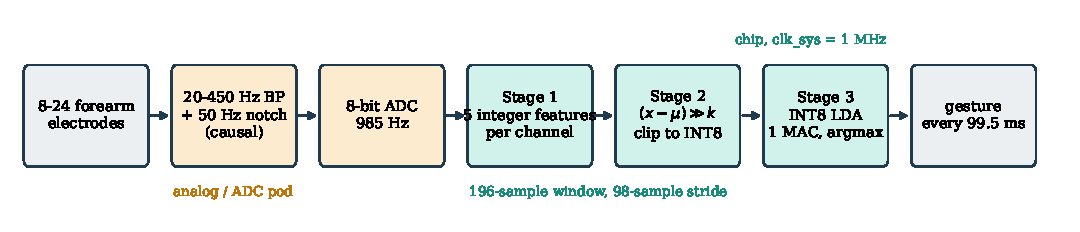
\includegraphics[width=\textwidth]{figures/pipeline.pdf}
\captionof{figure}{The classifier. The electrode pods filter and digitise the signal; the chip computes five
integer features per channel, normalises them with a shift, and an INT8 LDA decides one of four gestures every
98 samples (about 100\,ms).}\label{fig:pipeline}
\end{center}

%==========================================================================================
\section{Introduction}
Myoelectric control turns the electrical activity of forearm muscles into commands for a prosthetic hand, an
orthosis or a gesture interface. The signal is measured with surface electrodes on the skin, so it is cheap and
non-invasive; the price is that it is weak, noisy and different for every person. A practical controller has
to satisfy three requirements at once.
\begin{enumerate}
\item \textbf{It must work for a new user.} Skin and fat thickness, electrode placement and muscle physiology
change the signal from person to person. A classifier that is accurate only on the people it was trained on is
of little use. We therefore report only \emph{subject-independent} accuracy.
\item \textbf{It must run continuously on a battery.} This favours integer arithmetic, few multiplications,
small memories and a slow clock.
\item \textbf{It must feel immediate.} The optimal delay between the user's intent and the device's response
is about 100--125\,ms~\cite{farrell2007}; we decide every 100\,ms.
\end{enumerate}
Pattern-recognition control with time-domain features and LDA has been the reference approach for three
decades~\cite{hudgins1993,englehart2003,scheme2011}. The questions this work answers are which parts of that
recipe survive the constraints above, what a larger model would add, and how to build the result so that it
scales from 8 to 24 electrodes without redesign.

\paragraph{Contributions.}
\begin{itemize}
\item A complete, subject-independent design study on FORS-EMG~\cite{forsemg} in which every choice
(gestures, classifier, arithmetic, features, normaliser, calibration) is backed by a paired test
(Sections~\ref{sec:gestures}--\ref{sec:calib}).
\item A direct comparison of \emph{dropping} gestures against \emph{merging} all twelve into fewer classes,
with the grouping chosen inside each fold from the training subjects only (Section~\ref{sec:merge}).
\item Evidence that a raw-signal CNN gains at most a few points over the LDA, before and after per-user
calibration, at three orders of magnitude more arithmetic (Sections~\ref{sec:cnn} and~\ref{sec:calib}).
\item A fully integer front end (add, compare, shift and a leading-one detector) that is non-inferior to
floating-point features (Section~\ref{sec:frontend}).
\item An exact decomposition of the LDA over a chain of identical boards that exchanges only $K-1$ partial
sums, with a self-configuring chain protocol, one 256\,kHz clock and one multiplier per board
(Section~\ref{sec:hw}).
\item Verification by a bit-exact golden model, a self-checking unit test, a mutation test and a whole-chip
test on real data for six board splits (Section~\ref{sec:verif}).
\end{itemize}

%==========================================================================================
\section{Background}\label{sec:background}
\paragraph{Features and LDA.} Hudgins \emph{et al.}~\cite{hudgins1993} introduced a small set of time-domain
(TD) features (mean absolute value, zero crossings, slope sign changes, waveform length) computed over short
windows, and Englehart and Hudgins~\cite{englehart2003} showed that these features with an LDA give a robust,
real-time controller with very little storage. Phinyomark \emph{et al.}~\cite{phinyomark2012} later showed that
many published TD features are redundant, which motivates our feature culling.
\paragraph{Generalisation and robustness.} Clinical use is limited less by accuracy on a fixed session than by
changes between users, sessions and arm positions~\cite{scheme2011}. The limb-position effect is
well documented~\cite{fougner2011}; FORS-EMG~\cite{forsemg} was recorded in three forearm orientations
precisely to study it.
\paragraph{Integer inference.} Symmetric INT8 weights with INT32 accumulators are the standard way to run
linear layers and neural networks without floating point~\cite{jacob2018}. Mitchell's logarithm
approximation~\cite{mitchell1962} gives cheap squares and products in hardware.

%==========================================================================================
\section{Dataset and evaluation protocol}\label{sec:protocol}
\paragraph{Data.} FORS-EMG~\cite{forsemg} contains 19 subjects, 8 forearm electrodes sampled at 985\,Hz,
12 gestures, 3 forearm orientations (rest, supination, pronation) and 5 trials per gesture and orientation.
Each recording has 8000 samples (8.1\,s). Every gesture class pools all three orientations.
Figure~\ref{fig:signals} shows one recording of each of the four gestures finally used.

\paragraph{Signal chain.} A fourth-order Butterworth band-pass (20--450\,Hz) and a 50\,Hz notch ($Q=30$),
run \emph{causally} as cascaded biquads, because hardware cannot use future samples. Early experiments used
zero-phase filtering; every result that bears on the chip uses the causal filter. The filter removes baseline
drift and the mains line and keeps the EMG band (Figure~\ref{fig:spectrum}).

\paragraph{Windows.} 200\,ms windows (196--197 samples) with a 100\,ms stride, so consecutive windows share
half their samples. The chip uses exactly 196 samples (two banks of 98, Section~\ref{sec:board}).

\paragraph{Split.} Leave-one-subject-out (LOSO): in each fold one subject is held out and never used for
training, normalisation, quantisation scales or any other choice. Within the training subjects, trials 1--4
train and trial 5 validates. Windows are cut \emph{after} the split. An early version cut windows first;
because neighbouring windows overlap, validation windows leaked into training and produced a false accuracy
ceiling of about 63\% that did not depend on model capacity.

\paragraph{Statistics.} Accuracy is the mean over held-out subjects with a 95\% confidence interval (Student
$t$). Two methods are compared subject by subject: the mean paired difference, its 95\% interval, the
Wilcoxon signed-rank $p$-value and the number of subjects up and down. A difference is called real only if its
interval excludes zero; non-inferiority uses a margin of $-1$\pp.

\paragraph{Subject count.} The copy of the dataset in the project repository lacks subject~1. Runs made from it
use 18 subjects; runs on the full dataset use 19. Each table states which.

\begin{figure}[t]\centering
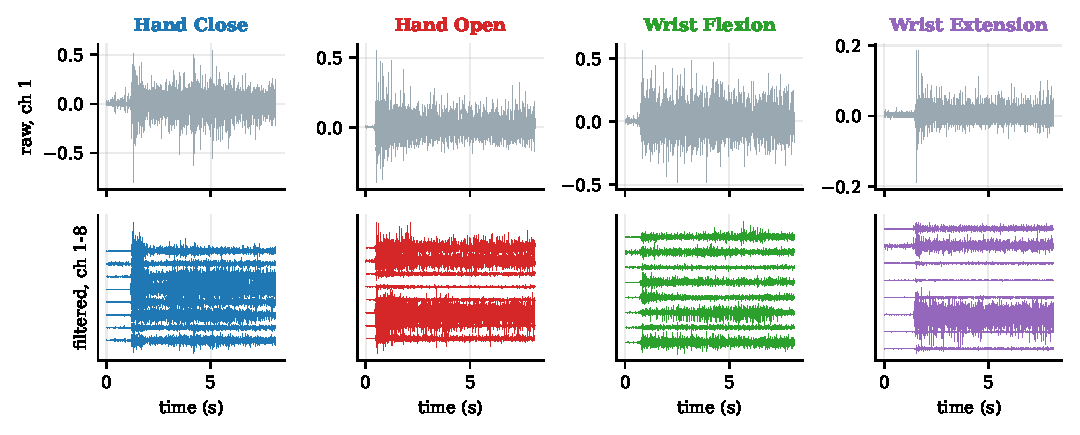
\includegraphics[width=\textwidth]{figures/signals.pdf}
\caption{One recording of each chosen gesture (subject 2, rest orientation). Top: raw channel 1. Bottom: all
eight channels after the causal filter. The gestures differ mainly in \emph{which} channels are active, which is
what per-channel amplitude features capture.}\label{fig:signals}
\end{figure}

\begin{figure}[t]\centering
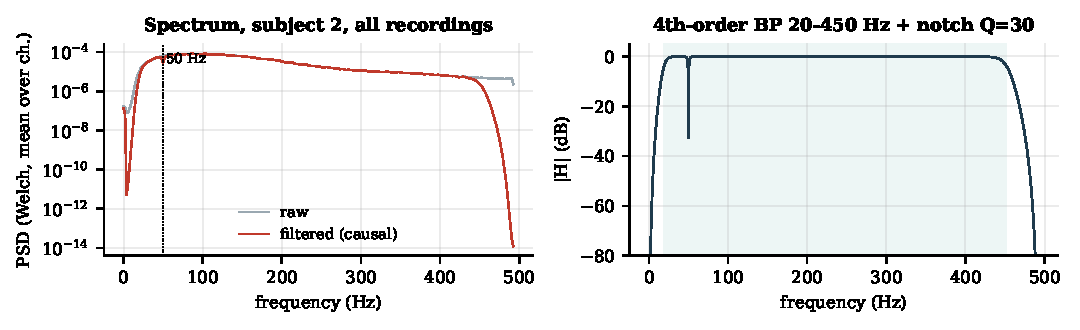
\includegraphics[width=0.9\textwidth]{figures/spectrum.pdf}
\caption{Left: power spectrum before and after the causal filter. Right: the filter's magnitude response.}
\label{fig:spectrum}
\end{figure}

%==========================================================================================
\section{Which gestures, and how many}\label{sec:gestures}
\subsection{Gesture kinds}
The twelve FORS-EMG gestures are of three kinds, driven by different muscles: whole-hand movements (Hand
Close, Hand Open), wrist movements (flexion, extension, radial and ulnar deviation), and finger postures
(Index, Index-Little, Peace, Thumb Up, Thumb-Little, Right Angle). Whole-hand and wrist movements use large,
superficial muscles; finger postures use the deep, overlapping compartments of the finger flexors, which eight
surface electrodes see only weakly.

Our first set, A = \{Hand Close, Hand Open, Index, Index-Little\}, stopped at about 65\% for every model.
Its confusion matrix showed that Index $\leftrightarrow$ Index-Little alone caused about 40\% of all errors.
Set B = \{Hand Close, Hand Open, Wrist Flexion, Wrist Extension\} replaces the two finger postures with two
wrist movements and gains $+14.1$\pp\ (paired $t$-test, 95\% interval $[+11.3,+16.9]$,
$p=3.8\times10^{-9}$), more than any later model or hardware choice (Table~\ref{tab:vocab},
Figure~\ref{fig:gestures}).

\paragraph{How many gestures.} Larger vocabularies cost accuracy. To find the best six, we ranked all
$\binom{12}{6}=924$ subsets by their worst confused pair in the 12-class confusion matrices. The best subset
(set D) was predicted at 66.4\% before training and measured at 69.0\%; all twelve gestures give 48.8\%.
In set D, Right Angle alone caused 44.5\% of the errors. With twelve classes, the MLP and logistic regression
agreed on nine of their ten most confused pairs, so the errors come from the signals, not from the model.

\begin{table}[t]\centering\small
\caption{Accuracy by gesture set (LOSO, 19 subjects, 64 floating-point features).}\label{tab:vocab}
\begin{adjustbox}{max width=\textwidth}
\begin{tabular}{llrrrrr}\toprule
Set & Model & FP32 \% & INT8 \% & INT8 loss (pp) & MACs & Bytes\\\midrule
A (4, hand + finger) & MLP 64-4 & 65.17 & 65.28 & $-0.12$ & 256 & 272\\
\hl B (4, hand + wrist) & MLP 64-16-4 & 79.69 & 79.38 & 0.32 & 1088 & 1168\\
\multirow{2}{*}{D (6)} & MLP 64-16-6 & 69.23 & 69.21 & 0.02 & 1120 & 1208\\
 & Logistic reg. & 68.95 & 68.74 & 0.21 & 384 & 408\\
\multirow{2}{*}{C (12)} & MLP 64-16-12 & 48.99 & 48.37 & 0.63 & 1216 & 1328\\
 & Logistic reg. & 49.71 & 49.28 & 0.43 & 768 & 816\\\bottomrule
\end{tabular}
\end{adjustbox}
\end{table}

\begin{figure}[t]\centering
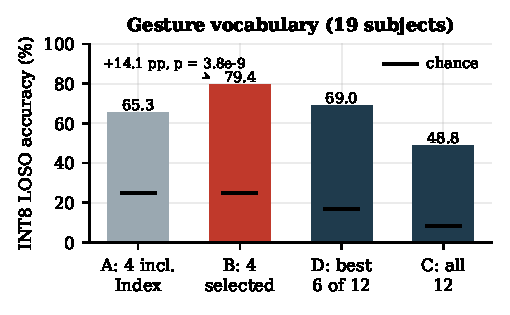
\includegraphics[width=0.55\textwidth]{figures/gesture_sets.pdf}
\caption{INT8 accuracy by gesture set (19 subjects); black bars mark chance.}\label{fig:gestures}
\end{figure}

\subsection{Merging all twelve gestures instead of dropping eight}\label{sec:merge}
Dropping eight gestures leaves two thirds of the recordings unused. The alternative is to keep every gesture
and merge them into four classes. To compare the two fairly we used the chip pipeline of
Section~\ref{sec:frontend} (8-bit ADC, streamed 196-sample windows, integer features, shift normaliser, INT8
LDA) for both.

\paragraph{Choosing the grouping without the test subject.} Inside each outer fold, a 12-class LDA is
cross-validated over the training subjects only (three folds of subjects), giving a $12\times12$ confusion
matrix $N$. Among all $12!/(3!^4\,4!)=15{,}400$ ways to split the gestures into four groups of three, we
choose the split $\mathcal{G}$ that maximises the share of windows predicted inside their own group,
\begin{equation}
\mathcal{G}^\star=\arg\max_{\mathcal{G}}\;\frac{1}{\sum_{ij}N_{ij}}\sum_{g\in\mathcal{G}}\;\sum_{i\in g}\sum_{j\in g}N_{ij}.
\end{equation}
Groups of equal size keep the classes balanced and stop the search from lumping every hard gesture into one
large class. The merged model is evaluated in two ways: a four-class LDA trained on the merged labels (same
chip), and the 12-class LDA whose decision is mapped to its group (three times the class rows). We also
evaluate the fixed six-group map used in an earlier stage of the project (G1 = Hand Close, Index,
Index-Little, Peace, Right Angle, Thumb Up; G2 = Hand Open, Wrist Extension; G3--G6 = Radial Deviation,
Thumb-Little, Ulnar Deviation, Wrist Flexion).

\begin{table}[t]\centering\small
\caption{Dropping versus merging (LOSO, 19 subjects, chip INT8 LDA). The paired difference is against
dropping.}\label{tab:merge}
\begin{adjustbox}{max width=\textwidth}
\begin{tabular}{lcccc}\toprule
Approach & Gestures used & Class rows & Accuracy \% & vs drop (pp, 95\% CI, up/down)\\\midrule
\hl Drop to HC, HO, WF, WE & 4 of 12 & 4 & $77.82\pm4.10$ & ---\\
Merge, 4 groups of 3, 4-class LDA & all 12 & 4 & $60.91\pm4.55$ & $-16.9\ [-20.3,-13.6]$, 0/19\\
Merge, 4 groups of 3, 12-class mapped & all 12 & 12 & $63.07\pm5.07$ & $-14.8\ [-18.2,-11.3]$, 0/19\\
Earlier 6-group map, 6-class LDA & all 12 & 6 & $72.38\pm4.11$ & $-5.5\ [-8.0,-2.9]$, 1/18\\
Earlier 6-group map, 12-class mapped & all 12 & 12 & $70.71\pm4.62$ & $-7.1\ [-10.4,-3.9]$, 2/17\\
12 gestures, no merging & all 12 & 12 & $46.41\pm5.55$ & ---\\\bottomrule
\end{tabular}
\end{adjustbox}
\end{table}

\begin{figure}[t]\centering
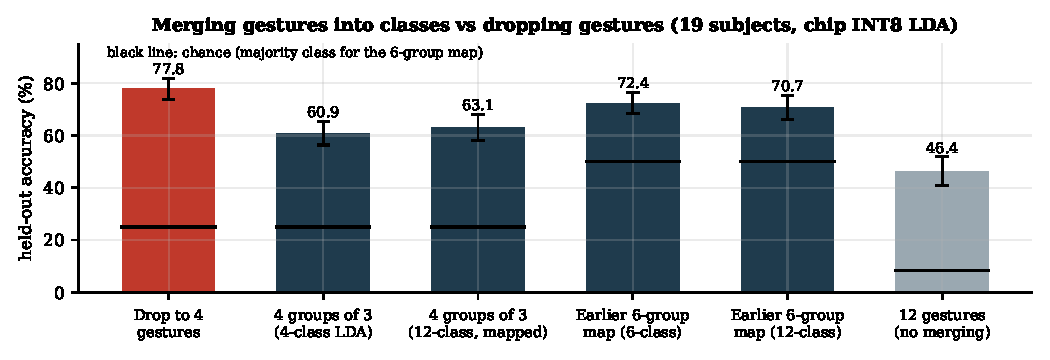
\includegraphics[width=0.95\textwidth]{figures/merge_drop.pdf}
\caption{Merging versus dropping. Bars: mean over 19 held-out subjects with 95\% intervals; black lines: chance
(for the six-group map, the share of the largest group, 50\%).}\label{fig:merge}
\end{figure}

\paragraph{Results.} Dropping wins on every subject (Table~\ref{tab:merge}, Figure~\ref{fig:merge}). The chosen
groupings are physiologically sensible: Hand Open and Wrist Extension fall into the same group in 19 of 19
folds, and Hand Close joins both thumb gestures in 17 of 19, while the groups of finger postures change from
fold to fold. Two effects explain the loss. First, the finger postures stay confusable however they are
grouped (twelve-class accuracy 46.4\%). Second, a merged class is a mixture of different muscle patterns,
which an LDA, with one Gaussian per class, fits poorly: mapping a 12-class decision to the groups beats training
on merged labels by $+2.2$\pp\ ($[+0.5,+3.8]$, $p=0.02$). The earlier six-group map reaches 72.4\%, but its
largest group holds half of all windows, so answering G1 every time already scores 50\%. \textbf{From here on
the classifier uses the four gestures of set B.}

\paragraph{A caveat on selection.} The ranking that chose set D, and the confusion data that confirmed set B,
came from LOSO confusion matrices that include the test subjects, which is mildly optimistic. The merge
experiment above chooses its groups inside each fold and is free of this bias. Set B was chosen first on
muscle grounds, and its 14\pp\ gain is far larger than any plausible selection effect.

%==========================================================================================
\section{Classifier}\label{sec:classifier}
\subsection{Eight classifiers on the same features}
All models in Table~\ref{tab:clf} see the same 64 floating-point features (eight TD types on eight channels),
the same folds and the same INT8 scheme, under a 10\,KB memory budget. The MLP has a ReLU hidden layer,
dropout 0.2, Adam with a cosine learning rate and early stopping on trial 5; the LDA uses a shared covariance
with Ledoit--Wolf shrinkage~\cite{ledoit2004}; trees have depth 10, forests 25 trees of depth 8, gradient
boosting 60 rounds of depth 4.

\begin{table}[t]\centering\small
\caption{Eight classifiers on set B (LOSO, 19 subjects). ``vs MLP'' is a paired test.}\label{tab:clf}
\begin{adjustbox}{max width=\textwidth}
\begin{tabular}{lrrrrrl}\toprule
Model & FP32 \% & INT8 \% & INT8 loss & MACs & Bytes & vs MLP\\\midrule
MLP 64-16-4 & 79.65 & 79.57 & 0.08 & 1088 & 1168 & ---\\
Gradient boosting & 79.63 & 79.26 & 0.37 & 0 & 19{,}200 & tied ($p=0.78$), over budget\\
Logistic regression & 79.33 & 79.19 & 0.14 & 256 & 272 & tied ($p=0.44$)\\
Linear SVM & 79.31 & 78.30 & 1.01 & 256 & 272 & tied ($p=0.29$)\\
\hl LDA & 77.91 & 77.87 & 0.04 & 256 & 272 & tied ($p=0.09$)\\
Random forest & 77.84 & 77.43 & 0.41 & 0 & 53{,}145 & worse ($p=0.046$)\\
Extra trees & 76.29 & 76.04 & 0.25 & 0 & 38{,}015 & worse ($p=0.0009$)\\
Decision tree & 73.69 & 73.17 & 0.52 & 0 & 5{,}055 & worse ($p=0.0002$)\\\bottomrule
\end{tabular}
\end{adjustbox}
\end{table}

The four linear-capacity models and the MLP are statistically tied; trees are worse or exceed the budget
(Figure~\ref{fig:clf}). On set A, five MLP widths from a single linear layer to 64-128-4 differ by 1.3\pp,
less than the $\pm5.9$\pp\ interval of any one of them, with 34 times the memory at the top
(Figure~\ref{fig:mlp}). The same tie between the MLP and logistic regression appears at 4, 6 and 12 gestures.
\textbf{Model capacity is not the bottleneck; the information in eight surface channels is.}

\begin{figure}[t]\centering
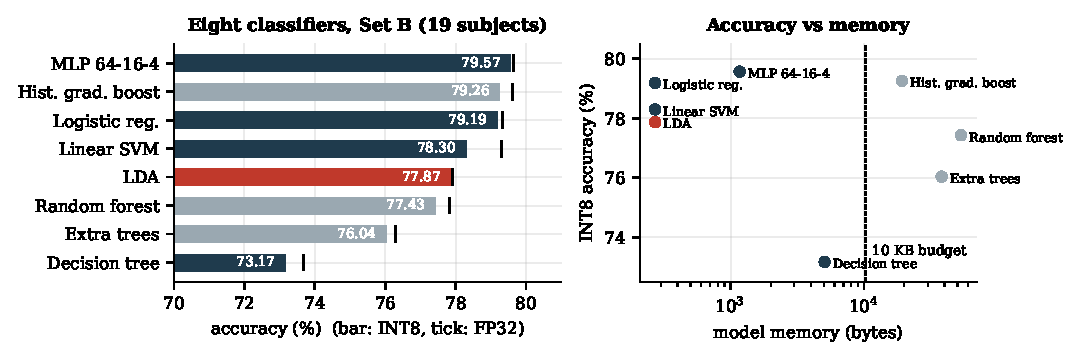
\includegraphics[width=\textwidth]{figures/classifiers.pdf}
\caption{Left: INT8 accuracy (bars) and FP32 accuracy (ticks) of the eight classifiers. Right: accuracy against
memory; grey models break the 10\,KB budget, red is the LDA used on the chip.}\label{fig:clf}
\end{figure}

\begin{figure}[t]\centering
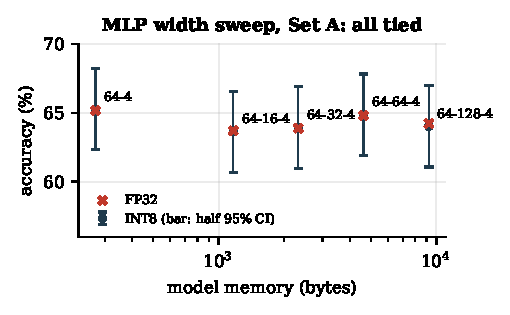
\includegraphics[width=0.5\textwidth]{figures/mlp_widths.pdf}
\caption{MLP width against memory on set A: 34 times the memory buys no accuracy.}\label{fig:mlp}
\end{figure}

\subsection{The LDA, and why we chose it}
With class means $\mu_k$, one shared covariance $\Sigma$ and priors $\pi_k$, the LDA assigns a feature vector
$q$ to the class with the largest linear score
\begin{equation}
s_k(q)=w_k^{\top}q+b_k,\qquad w_k=\Sigma^{-1}\mu_k,\qquad b_k=-\tfrac12\,\mu_k^{\top}\Sigma^{-1}\mu_k+\log\pi_k.
\label{eq:lda}
\end{equation}
Logistic regression had a slightly better point estimate, but we chose the LDA because:
(1)~its training is closed form (means and one covariance), so retraining for a new user or a new electrode
layout is a few matrix operations and no optimiser, which Section~\ref{sec:calib} exploits;
(2)~its weights are stored in writable memory, so a new model needs no new silicon;
(3)~its scores are log-likelihoods up to a shared constant.
It costs 1.7\pp\ against the MLP, inside the tie, for 4.3 times fewer multiply-accumulates (MACs) and bytes.

\subsection{INT8 arithmetic}\label{sec:quant}
Weights and activations are symmetric per-tensor INT8 with the scale set at the 99.9th percentile of the
magnitudes; biases are INT32 on the product scale $s_W s_x$, so they add directly into the accumulator. All
scales come from the training subjects. Over 28 FP32-versus-INT8 comparisons (every model and gesture set)
the loss is 0.18\pp\ on average (median 0.11, worst 1.01 for the linear SVM, whose hinge loss produces larger
weights), and 25 of 28 losses are below 0.5\pp\ (Figure~\ref{fig:qdrop}). A requantisation bug (a shift of
$\lceil-\log_2 M\rceil$, undefined for multipliers $M>1$) would have cost more than 50\pp; a synthetic unit test
caught it before any result was reported.

The chip needs no requantisation at all. Only the argmax is used, and if every class score shares one positive
scale $s$, then $\arg\max_k s\,S_k=\arg\max_k S_k$. The chip therefore keeps one INT32 accumulator per class and
one weight scale for all classes.

\begin{figure}[t]\centering
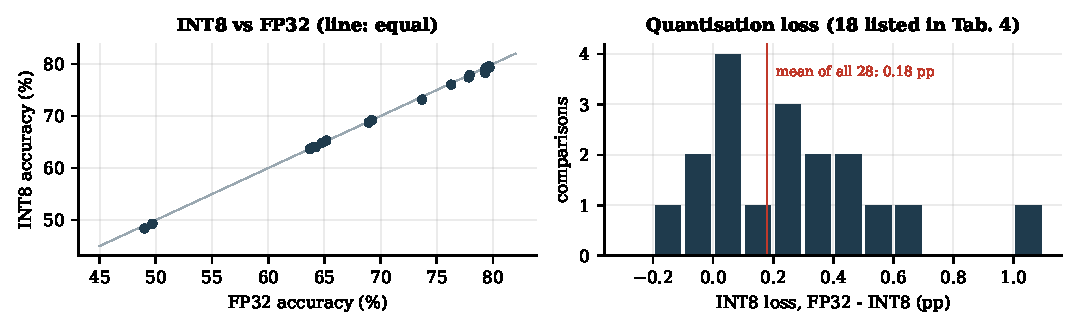
\includegraphics[width=\textwidth]{figures/qdrop.pdf}
\caption{INT8 against FP32 for the results of Tables~\ref{tab:vocab}--\ref{tab:clf} (left), and the
distribution of the losses (right).}\label{fig:qdrop}
\end{figure}

%==========================================================================================
\section{Features}\label{sec:features}
\subsection{Which feature types}
sEMG is noise-like: what separates gestures is how strongly and how fast each channel's signal varies, which is
exactly what TD features measure~\cite{hudgins1993,englehart2003}. We started from eight TD types per channel
(64 inputs) and selected types by nested LOSO on the INT8 LDA (18 subjects): for each held-out subject, all 127
subsets of seven candidate types were scored by an inner LOSO on the other 17 subjects, and the smallest subset
within one paired standard error of the best was kept. IEMG was excluded beforehand, because
IEMG $=N\cdot$MAV gives an identical LDA.

MAV, RMS, WL and VAR are almost the same signal (Spearman $|\rho|\ge0.977$, Figure~\ref{fig:featsel}), in
line with~\cite{phinyomark2012}; ZC, SSC and WAMP carry different information, but WAMP saturates (98\% of
sample differences exceed its threshold). The selected set \{MAV, WL, ZC, SSC, VAR\} reaches
$77.08\pm4.97\%$ against $77.31\pm5.02\%$ with all eight types ($\Delta=-0.23\pm0.42$\pp, $p=0.20$,
non-inferior), with 40 inputs instead of 64: 160 instead of 256 MACs and 176 instead of 272 bytes. MAV, ZC and
VAR were chosen in all 18 folds, WL in 17 and SSC in 14.

\begin{figure}[t]\centering
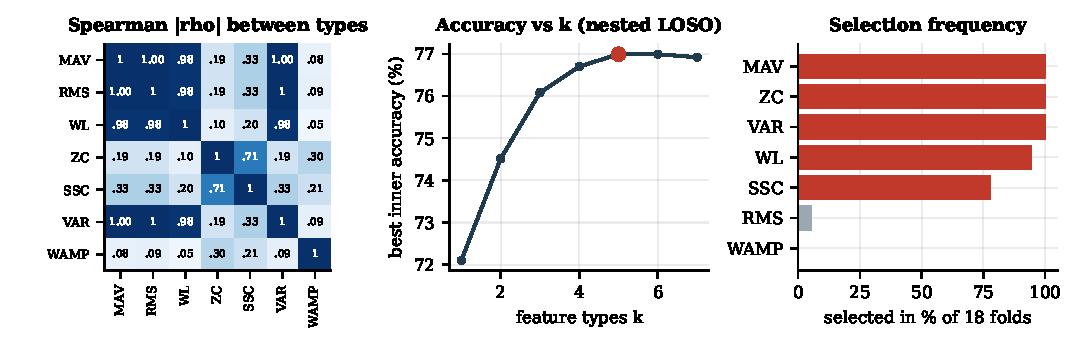
\includegraphics[width=\textwidth]{figures/feature_selection.pdf}
\caption{Feature-type selection. Left: rank correlation between types. Middle: best inner-LOSO accuracy for each
number of types. Right: how often each type was selected over the 18 outer folds.}\label{fig:featsel}
\end{figure}

\subsection{An integer-only front end}\label{sec:frontend}
The selected features need division, square roots and floating-point thresholds. We rebuilt them from add,
subtract, absolute value, compare, shift and a leading-one detector. For an 8-bit sample $x_n$ of one channel
and a window of $N$ samples:
\begin{align}
\text{SABS}&=\textstyle\sum_n |x_n|, & \text{WL}&=\textstyle\sum_n |x_n-x_{n-1}|,\\
\text{ZC}&=\textstyle\sum_n \big[\operatorname{sign}(x_n)\ne\operatorname{sign}(x_{n-1})\big], &
\text{SSC}&=\textstyle\sum_n \big[d_n d_{n-1}<0\big],\quad d_n=x_n-x_{n-1},\\
\text{POW}&=\textstyle\sum_n \widehat{a_n^2}, & \widehat{a^2}&=a\cdot2^{p+1}-2^{2p},\quad p=\lfloor\log_2 a\rfloor,\; a=|x_n|.
\end{align}
SABS replaces MAV (the factor $1/N$ is absorbed by the normaliser), ZC is a sign-bit XOR without a dead-band,
SSC counts strict changes of slope sign (only the sign of the previous difference is stored), and POW replaces
VAR.
The square in POW is Mitchell's one-step square~\cite{mitchell1962}: one leading-one detector, two shifts and one
subtraction. Writing $a=2^p(1+f)$ with $0\le f<1$ gives $a^2-\widehat{a^2}=2^{2p}f^2\ge0$, so it never
overestimates, is exact at powers of two and errs by at most 25\% (Figure~\ref{fig:mitchell}); the summed
feature still has correlation $r=0.9999$ with $\sum x^2$.

\begin{figure}[t]\centering
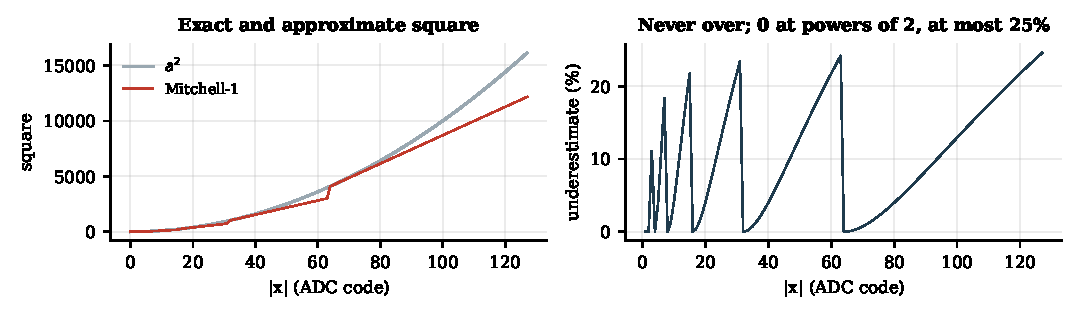
\includegraphics[width=\textwidth]{figures/mitchell.pdf}
\caption{Mitchell's square of an 8-bit magnitude: a smooth, monotone underestimate, so the window sum stays
almost perfectly correlated with the exact sum of squares.}\label{fig:mitchell}
\end{figure}

\paragraph{Shift normaliser.} Z-scoring and input quantisation are replaced by
\begin{equation}
q_f=\operatorname{clip}\Big(\big((x_f-\mu_f)+2^{k_f-1}\big)\gg k_f,\;-128,\;127\Big),
\end{equation}
with an integer $\mu_f$ (the rounded training mean) and the smallest $k_f\ge1$ that never clips on the training
subjects. The LDA is invariant to a positive rescaling of any one feature, so replacing the standard deviation
by a power of two costs nothing in principle; rounding and clipping are the only approximations. Count features
need $k=1$, amplitude features 4--6 and power features 7--12 (Figure~\ref{fig:norm}).

\begin{figure}[t]\centering
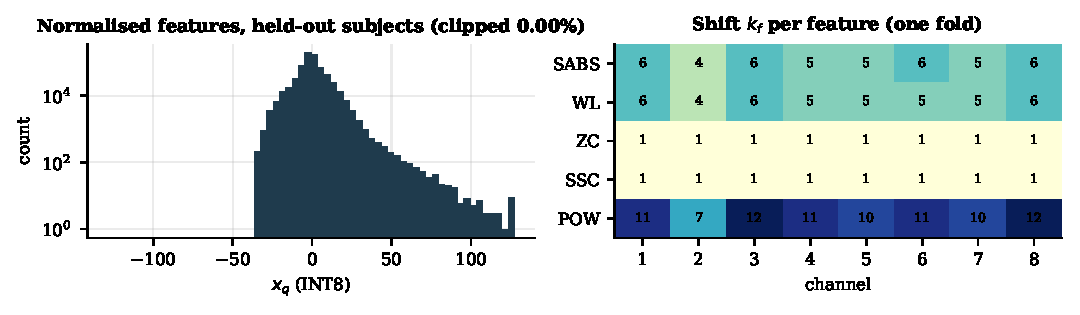
\includegraphics[width=\textwidth]{figures/normaliser.pdf}
\caption{Left: the INT8 inputs $q_f$ on held-out windows. Right: the shifts $k_f$ of one fold.}\label{fig:norm}
\end{figure}

\paragraph{Result.} Six integer variants were compared with the floating-point reference on the same folds
(Table~\ref{tab:hw}, Figure~\ref{fig:hw}). Every variant that keeps a power feature is non-inferior; dropping
power costs 1.9\pp\ and fails, so a power feature is needed; the shift normaliser costs nothing against
z-scoring. We chose H6, the cheapest variant. On 19 subjects the integer front end gives $77.79\pm4.39\%$
against 77.88\% for floating-point features.

\begin{table}[t]\centering\small
\caption{Integer feature variants, INT8 LDA, LOSO (18 subjects). $\Delta$: paired difference to the reference R,
with the shift normaliser.}\label{tab:hw}
\begin{adjustbox}{max width=\textwidth}
\begin{tabular}{llccc}\toprule
 & Power feature / ZC & Standard normaliser \% & Shift normaliser \% & $\Delta$ vs R (pp, 95\% CI)\\\midrule
R & floating-point reference & 77.45 & -- & --\\
H1 & exact $\sum x^2$ & 77.33 & 77.63 & $+0.19\,[-0.36,+0.73]$\\
H2 & Mitchell, two steps & 77.29 & 77.56 & $+0.11\,[-0.41,+0.63]$\\
H3 & Mitchell, one step & 77.26 & 77.39 & $-0.05\,[-0.57,+0.47]$\\
H4 & $(\sum|x|)^2$ & 77.10 & 77.14 & $-0.31\,[-0.88,+0.27]$\\
H5 & no power feature & 75.38 & 75.54 & $-1.91\,[-2.94,-0.87]$\\
\hl H6 & Mitchell, one step; ZC without dead-band & 77.29 & 77.39 & $-0.05\,[-0.59,+0.48]$\\\bottomrule
\end{tabular}
\end{adjustbox}
\end{table}

\begin{figure}[t]\centering
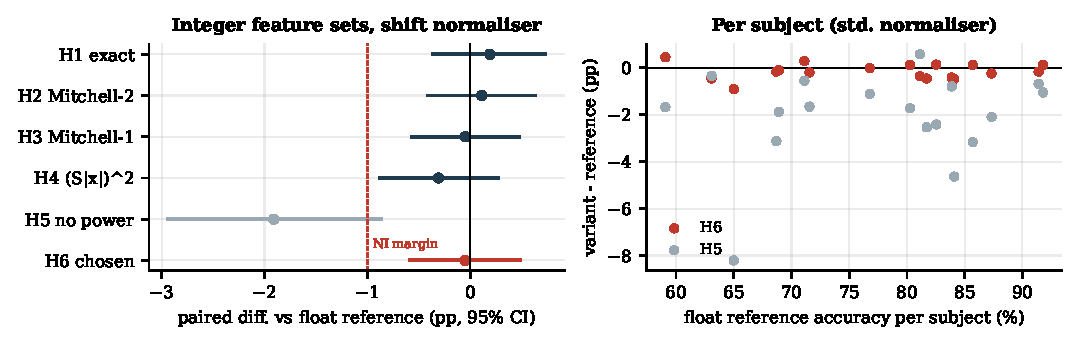
\includegraphics[width=\textwidth]{figures/hw_variants.pdf}
\caption{Left: paired difference of each integer variant to the floating-point reference; the dashed line is the
non-inferiority margin. Right: per-subject differences for H6 and for H5, which drops the power feature.}
\label{fig:hw}
\end{figure}

\subsection{The chip's own numbers}
A golden model reproduces every integer of the chip: an 8-bit ADC, recordings streamed sample by sample (so WL,
ZC and SSC use the true previous sample), 196-sample windows from two banks, the shift normaliser and an INT8
LDA with one weight scale. Trained and tested by LOSO on its own bit-exact features, it reaches
$77.61\pm4.34\%$ against $77.83\pm4.11\%$ for the software INT8 LDA: $\Delta=-0.21$\pp, $[-0.72,+0.30]$,
$p=0.49$, nine subjects up and nine down (Figure~\ref{fig:persub}). There is no detectable cost to the chip's
arithmetic. The value ranges leave wide margins: $\mu_f$ uses at most 13 of its 22 bits, $k_f\in[1,12]$, scores
stay below 4047 in magnitude against the INT32 limit, and no feature clips.

Most remaining errors are Wrist Extension predicted as Hand Open (29\%) and the reverse (18\%)
(Figure~\ref{fig:confusion}): the two movements share extensor-digitorum activity.

\begin{figure}[t]\centering
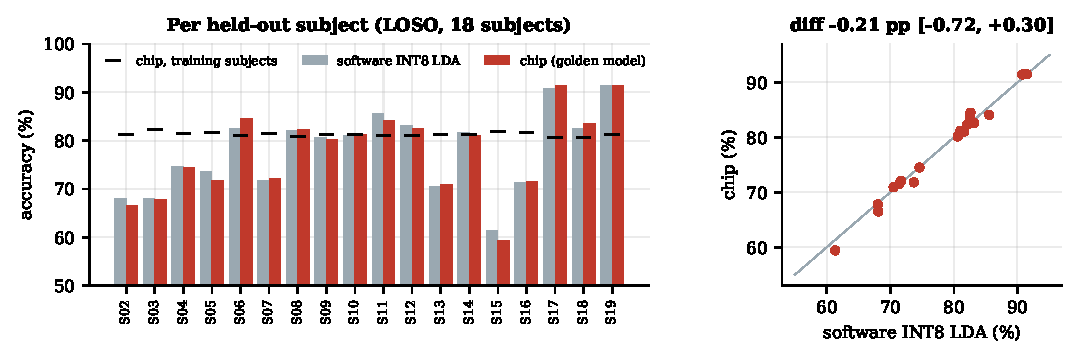
\includegraphics[width=\textwidth]{figures/per_subject.pdf}
\caption{Held-out accuracy of the chip model and the software INT8 LDA per subject; the points lie on the
diagonal.}\label{fig:persub}
\end{figure}

\begin{figure}[t]\centering
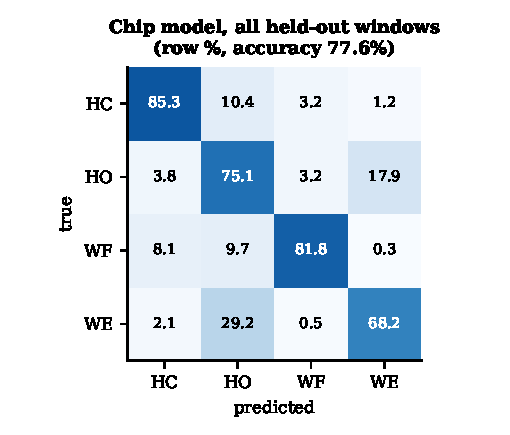
\includegraphics[width=0.45\textwidth]{figures/confusion.pdf}
\caption{Confusion matrix of the chip model over all held-out windows of all folds (row \%).}
\label{fig:confusion}
\end{figure}

%==========================================================================================
\section{Would a convolutional network do better?}\label{sec:cnn}
If the features carry the information, a network that learns its own features from the raw signal might find
what our five types miss. Two raw-signal CNNs were trained on exactly the same windows and folds as the LDA.
Every convolution is a 1-D convolution with batch normalisation and ReLU.
\begin{itemize}
\item \textbf{Option 2 (depthwise-separable).} A depthwise temporal convolution ($8\to32$, kernel 15, four
filters per electrode), a pointwise mix ($32\to32$), three separable blocks with stride 2
($32\to48\to64\to64$), global average pooling and a $64\to4$ output layer.
\item \textbf{Option 5c (two-branch).} A temporal branch (depthwise, kernel 15) and a spatial branch
(pointwise $8\to32$) in parallel, concatenated to 64 channels, then two separable blocks, pooling and the
output layer.
\end{itemize}
Training uses AdamW, a cosine learning rate, label smoothing 0.1, dropout 0.3, at most 150 epochs and early
stopping on trial 5 (patience 20). Each electrode of each training window is multiplied by a random gain
$e^{z}$, $z\sim\mathcal{N}(0,0.3^2)$, imitating differences in skin contact between people. For INT8, batch
normalisation is folded into the convolution weights.

\begin{table}[t]\centering\small
\caption{Raw-signal CNNs against the LDA (LOSO, 19 subjects, INT8). The paired difference is against the LDA.}
\label{tab:cnn}
\begin{adjustbox}{max width=\textwidth}
\begin{tabular}{lrrcc}\toprule
Model & MACs / decision & Parameters & Accuracy \% & vs LDA (pp, 95\% CI, up/down)\\\midrule
\hl LDA, 40 integer features & 160 & 164 & $77.79\pm4.39$ & ---\\
CNN option 2 & 751{,}584 & 11{,}732 & $79.10\pm4.10$ & $+1.31\ [-1.00,+3.61]$, 14/5, $p=0.20$\\
CNN option 5c & 594{,}400 & 12{,}132 & $80.48\pm3.81$ & $+2.68\ [+0.76,+4.61]$, 15/4, $p=0.008$\\\bottomrule
\end{tabular}
\end{adjustbox}
\end{table}

\begin{figure}[t]\centering
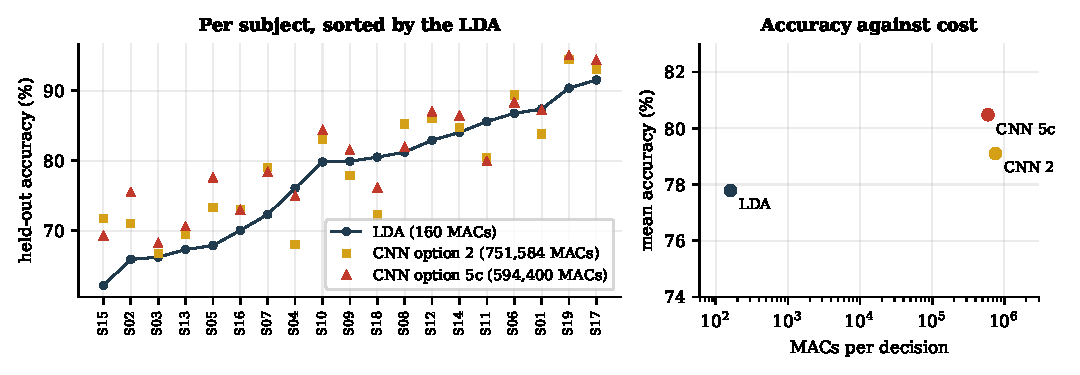
\includegraphics[width=\textwidth]{figures/cnn_lda.pdf}
\caption{Left: per-subject accuracy of the LDA and the two CNNs, sorted by the LDA. Right: mean accuracy against
MACs per decision (log scale).}\label{fig:cnn}
\end{figure}

The separable CNN is not distinguishable from the LDA; the two-branch CNN is better by 2.7\pp\ on 15 of 19
subjects (Table~\ref{tab:cnn}, Figure~\ref{fig:cnn}). INT8 changes neither network measurably. The gain
costs about 3{,}700 times the MACs and 74 times the parameters. A network that learns its features from raw
samples finds only a little that the TD features miss, which is the same conclusion as the classifier comparison
from a different direction: with eight surface electrodes, the signal, not the model, sets the limit.

%==========================================================================================
\section{Per-user calibration}\label{sec:calib}
The global model has never seen the user; it reaches about 78\% on average and under 60\% for the worst user.
A short recording of the user, one repetition of each gesture (about 8\,s each), can adapt it.

\subsection{Calibrating the LDA}
Because the LDA is closed form, calibration only blends statistics. With the global class means
$\mu_k^{g}$ and covariance $\Sigma^{g}$, and the same quantities $\mu_k^{u},\Sigma^{u}$ estimated from the
user's recording,
\begin{equation}
\mu_k\leftarrow(1-\lambda)\,\mu_k^{g}+\lambda\,\mu_k^{u},\qquad
\Sigma\leftarrow(1-\lambda)\,\Sigma^{g}+\lambda\,\Sigma^{u},
\end{equation}
and $w_k,b_k$ are recomputed from Equation~\eqref{eq:lda}: one $40\times40$ solve. The new weights are quantised
and written to the chip over its configuration port; no hardware change is needed. With $\lambda=0.5$,
calibration on trial 1 and testing on trials 3--5 of each held-out subject (never used for calibration), the
INT8 LDA rises from $78.03\pm4.76\%$ to $86.35\pm2.56\%$ on 18 subjects: $+8.3$\pp\ ($[+4.4,+12.3]$),
all 18 subjects improve, Wilcoxon $p=2\times10^{-4}$ (Figure~\ref{fig:calib}, left). The worst users gain most
(S15 $+30.1$\pp, S13 $+20.1$\pp), so the spread between users halves. A second calibration trial adds only
0.4\pp.

\subsection{Calibrating a CNN, and the decision}
A dedicated study (the project's CNN checkpoint) compared the two families after calibration on all 19
subjects, with three training seeds per CNN and five rounds per subject in which every trial serves once each
as test, validation and calibration data. Its setting differs from the rest of this paper: all twelve gestures
are classified and mapped to the six groups of Section~\ref{sec:merge}, 150\,ms windows with a 50\,ms stride are
used, only windows after the first 0.5\,s of each recording (the gesture is held) are scored, and the LDA is
calibrated by first re-centring the features on the user's gestures and then blending with the global statistics,
with the blend chosen on validation. Five ways of calibrating a CNN were compared; only retraining all weights
(learning rate 0.001, 20 epochs, chosen on validation) beat the LDA.

\begin{table}[t]\centering\small
\caption{CNN checkpoint: group accuracy (six groups) on held windows, INT8, 19 subjects.}\label{tab:calib}
\begin{adjustbox}{max width=\textwidth}
\begin{tabular}{lccccc}\toprule
Model & No calibration & 1 trial ($\approx$5\,min) & 2 trials & 3 trials & Gain from 1 trial\\\midrule
LDA (re-centre + blend) & 71.4 & 91.9 & 92.7 & 93.1 & $+20.5$\\
CNN ``small'' (49k MACs) & 75.4 & 92.2 & -- & -- & $+16.9$\\
CNN ``two'' (452k MACs) & 78.1 & 94.3 & 95.2 & 95.9 & $+16.2$\\\bottomrule
\end{tabular}
\end{adjustbox}
\end{table}

\begin{figure}[t]\centering
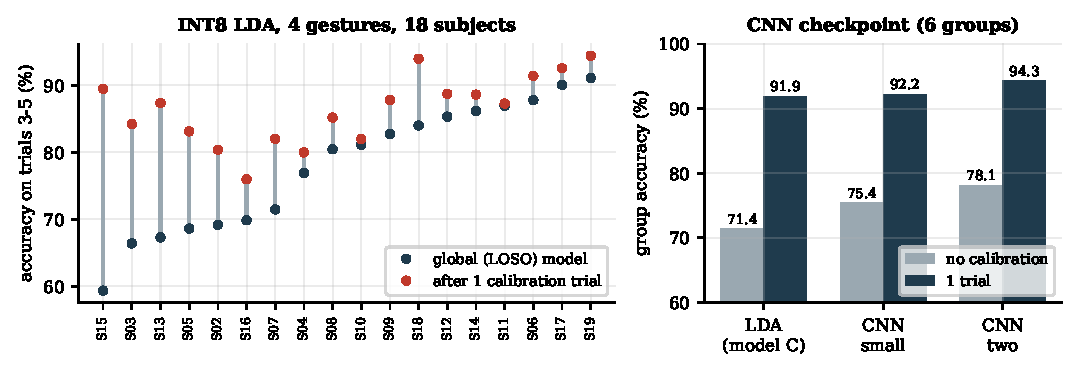
\includegraphics[width=\textwidth]{figures/calibration.pdf}
\caption{Left: LDA accuracy per subject before and after one calibration trial (four gestures, 18 subjects).
Right: the CNN checkpoint, before and after one calibration trial.}\label{fig:calib}
\end{figure}

After one trial the larger CNN leads by $+2.39$\pp\ ($[+1.87,+2.90]$), better for all 19 subjects; the
smaller CNN is level with the LDA ($+0.32$, $[-0.13,+0.76]$). Calibration closes most of the CNN's head start
($+6.7$\pp\ before, $+2.4$\pp\ after), because what the CNN does better, coping with differences between
people, is exactly what calibration corrects. The CNN's advantages are real: with one trial it beats the LDA
with three, and when calibrated in only one arm position it loses 9.6\pp\ against the LDA's 12.1\pp\ (both
models still need calibration across positions, as expected from the limb-position effect~\cite{fougner2011}).
But the adoption bar fixed before the study was $+3$\pp, and the larger CNN needs about 870 times the LDA's
arithmetic, a clock of at least 9\,MHz, and retraining of about 12{,}000 weights at every calibration instead of a
closed-form blend. \textbf{We keep the LDA.}

%==========================================================================================
\section{Hardware}\label{sec:hw}
\subsection{From one chip to a chain of boards}
Our first chip served 8 to 24 electrodes from one compute core and up to three 8-channel ADC pods, with a 1\,MHz
core clock, an 8\,MHz SPI clock and a synchroniser between them. Its memories had to be sized for 24 channels
(13.5\,kbit) even when only 8 were used, and its Stage 2 and 3 took up to 850 of the 1015 cycles of a sample
period. The final design instead makes every board identical: one 8-channel pod and one chip. Each board
computes features, normalisation and its share of the LDA on its own channels; boards are chained, and only
three partial sums per decision cross between them (Figure~\ref{fig:system}). Compute grows with the number of
boards, so one slow clock suffices, and a board needs only 3.7\,kbit of memory.

\begin{figure}[t]\centering
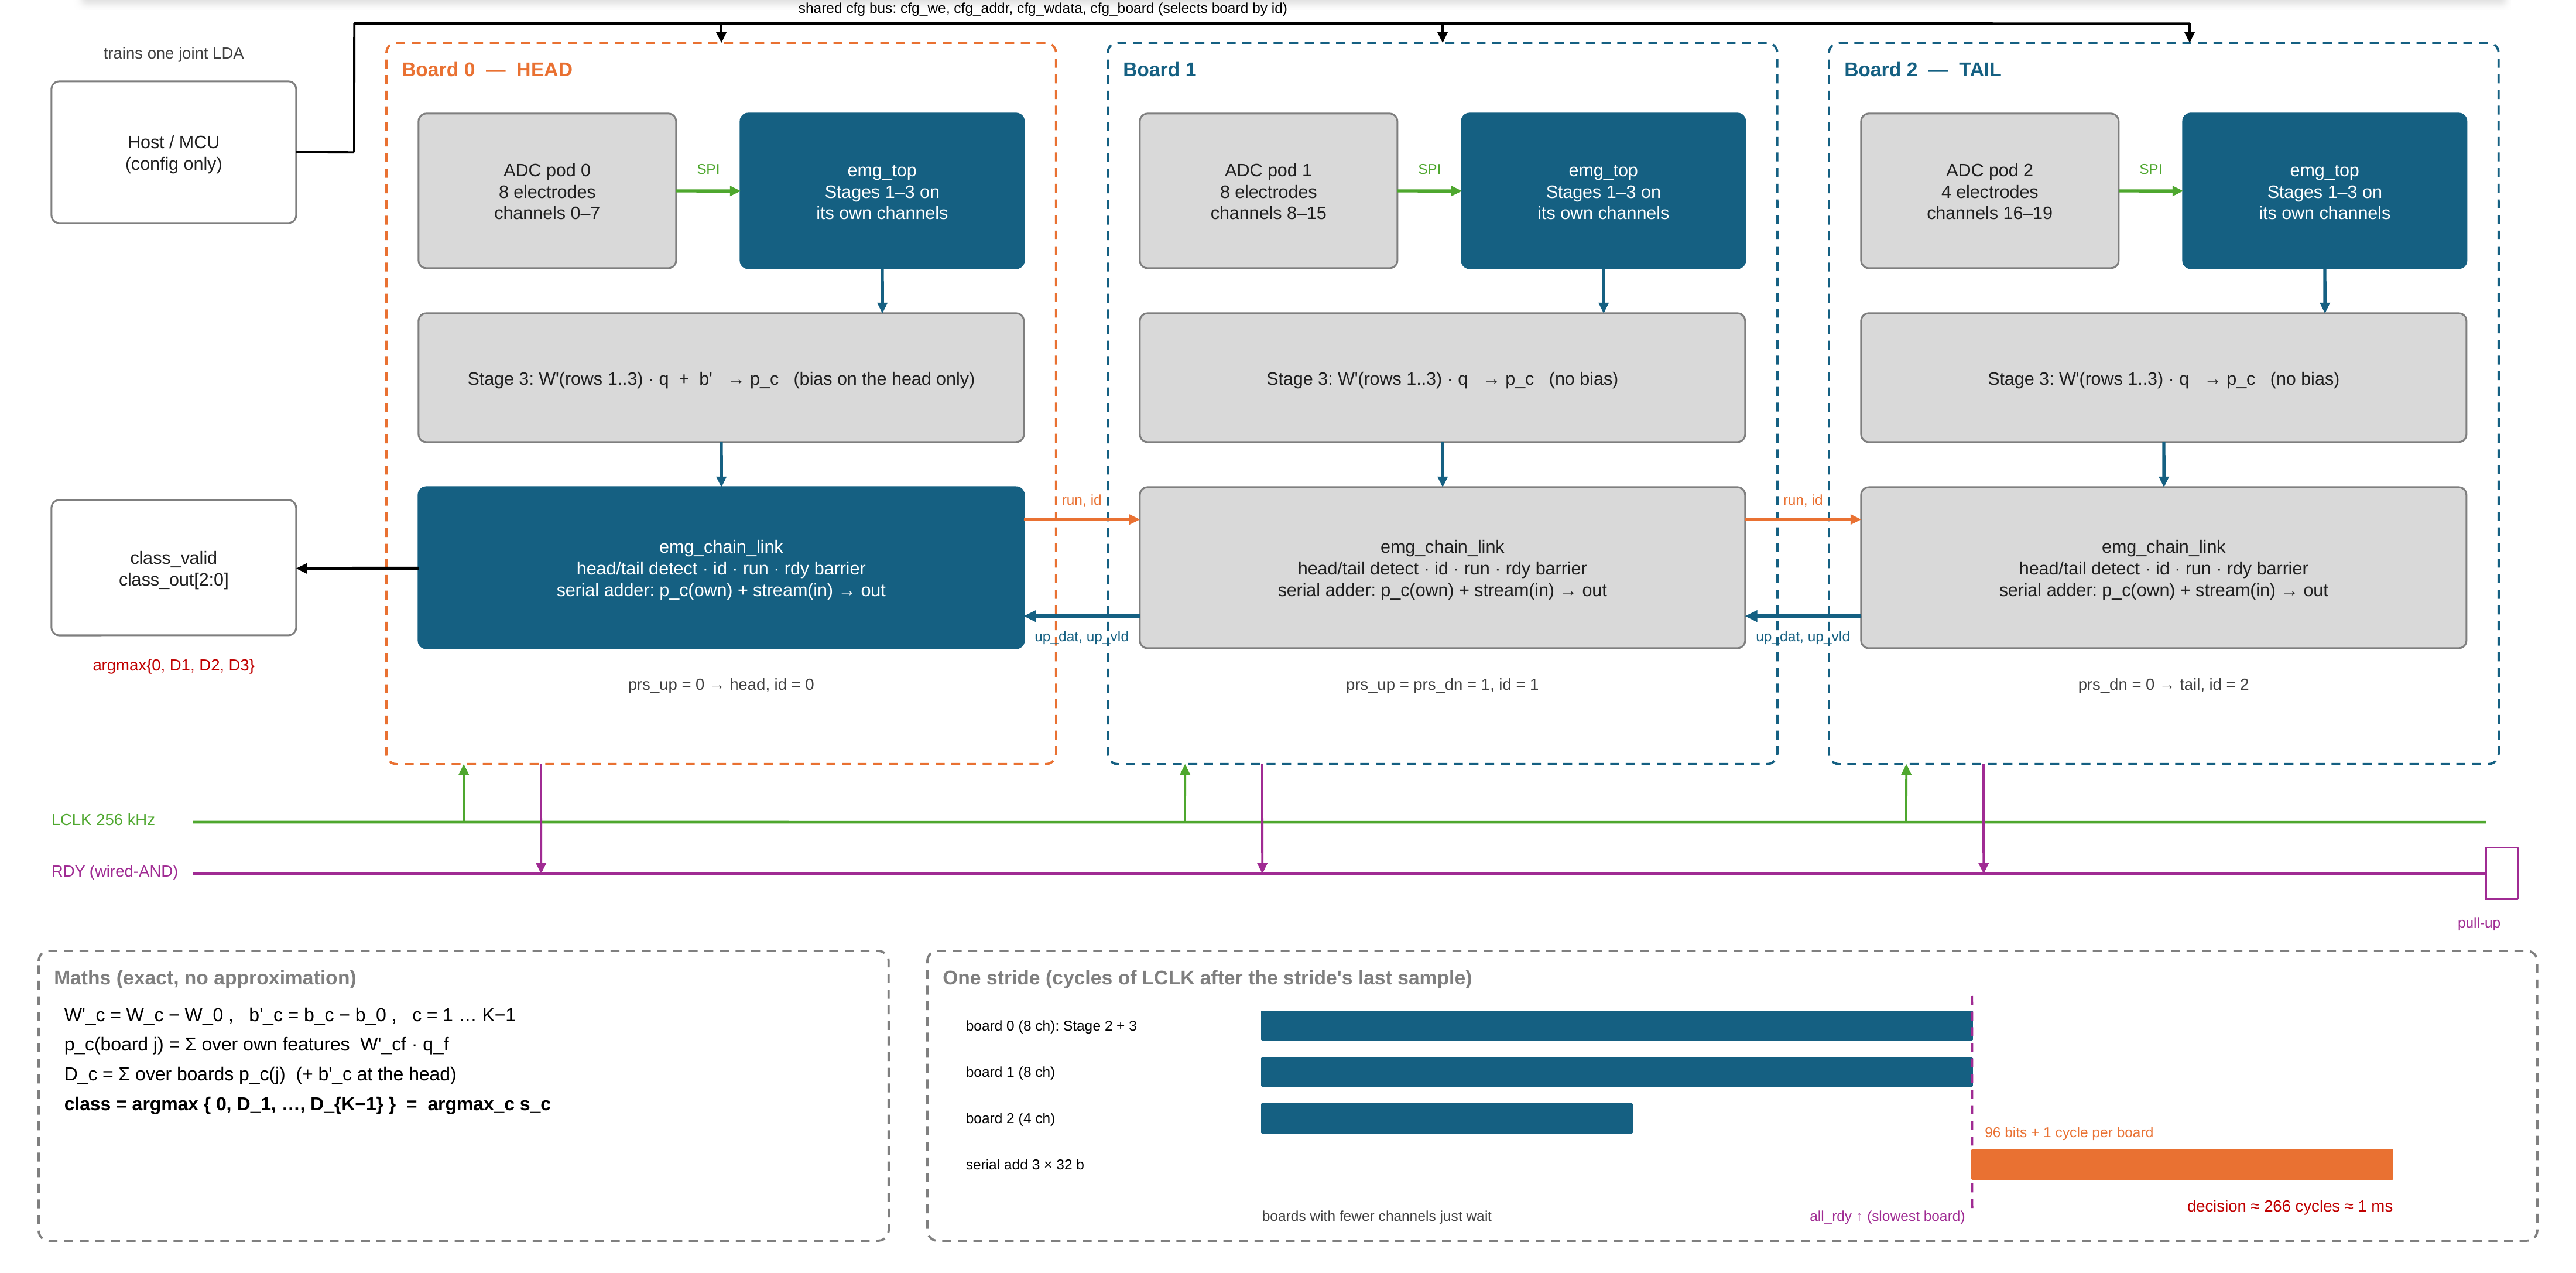
\includegraphics[width=\textwidth]{figures/system.png}
\caption{The multi-board system: three boards in a chain (8 + 8 + 4 electrodes), a shared configuration bus, one
256\,kHz clock and a wired-AND ready line. Only the partial sums $p_c$ travel along the chain, towards the
head.}\label{fig:system}
\end{figure}

\subsection{One board}\label{sec:board}
Figure~\ref{fig:board} shows a board's datapath with the RTL module names.
\begin{enumerate}
\item \textbf{ADC interface} (\texttt{emg\_spi\_adc}). A timer issues CONVST every 260 cycles; after the pod's
data-ready signal, an SPI burst reads 64 bits (eight channels of 8 bits) at half the clock rate.
\item \textbf{Stage 1, features} (\texttt{emg\_feat\_accum}, \texttt{emg\_feat\_alu}). For each new frame, a
two-stage pipeline reads one channel's history (the previous sample and the sign of the previous difference,
10 bits) and its bank word, computes the five feature increments combinationally and writes the sums back: one
channel per cycle, $C\le8$ cycles per sample.
\item \textbf{Windows.} Two ping-pong banks each accumulate 98 samples. A window is the sum of the two banks, so
each completed bank finishes a 196-sample window with a 98-sample stride, using one write pointer and no
sliding subtraction (Figure~\ref{fig:banks}). The first decision after reset is masked, because only one bank
is full.
\item \textbf{Stage 2, normaliser} (\texttt{emg\_shift\_norm}). After every 98th sample it adds the two bank
fields, subtracts $\mu_f$, rounds, shifts by $k_f$ and clips, for $f=0,\dots,D-1$: $D+2$ cycles.
\item \textbf{Stage 3, LDA} (\texttt{emg\_lda\_mac}). One signed $8\times8$ multiplier and an INT32
accumulator. For each of the $K-1=3$ rows it loads the bias and performs $D$ MACs: $3(D+1)+2$ cycles.
\item \textbf{Chain link} (\texttt{emg\_chain\_link}). Position and identity, the common start, the barrier,
the bit-serial adder and, on the head, the running argmax (Section~\ref{sec:chain}).
\end{enumerate}
All constants ($\mu_f,k_f$, the weight rows and biases) live in writable RAM, because every electrode layout and
every calibrated user needs its own model. Every memory has a one-cycle synchronous read, so the RTL maps to SRAM
macros or flip-flops unchanged. A board holds 3{,}656 bits: banks 1{,}024, $\mu,k$ 1{,}080, weights 960, INT8
features 320, biases 192 and history 80.

\begin{figure}[t]\centering
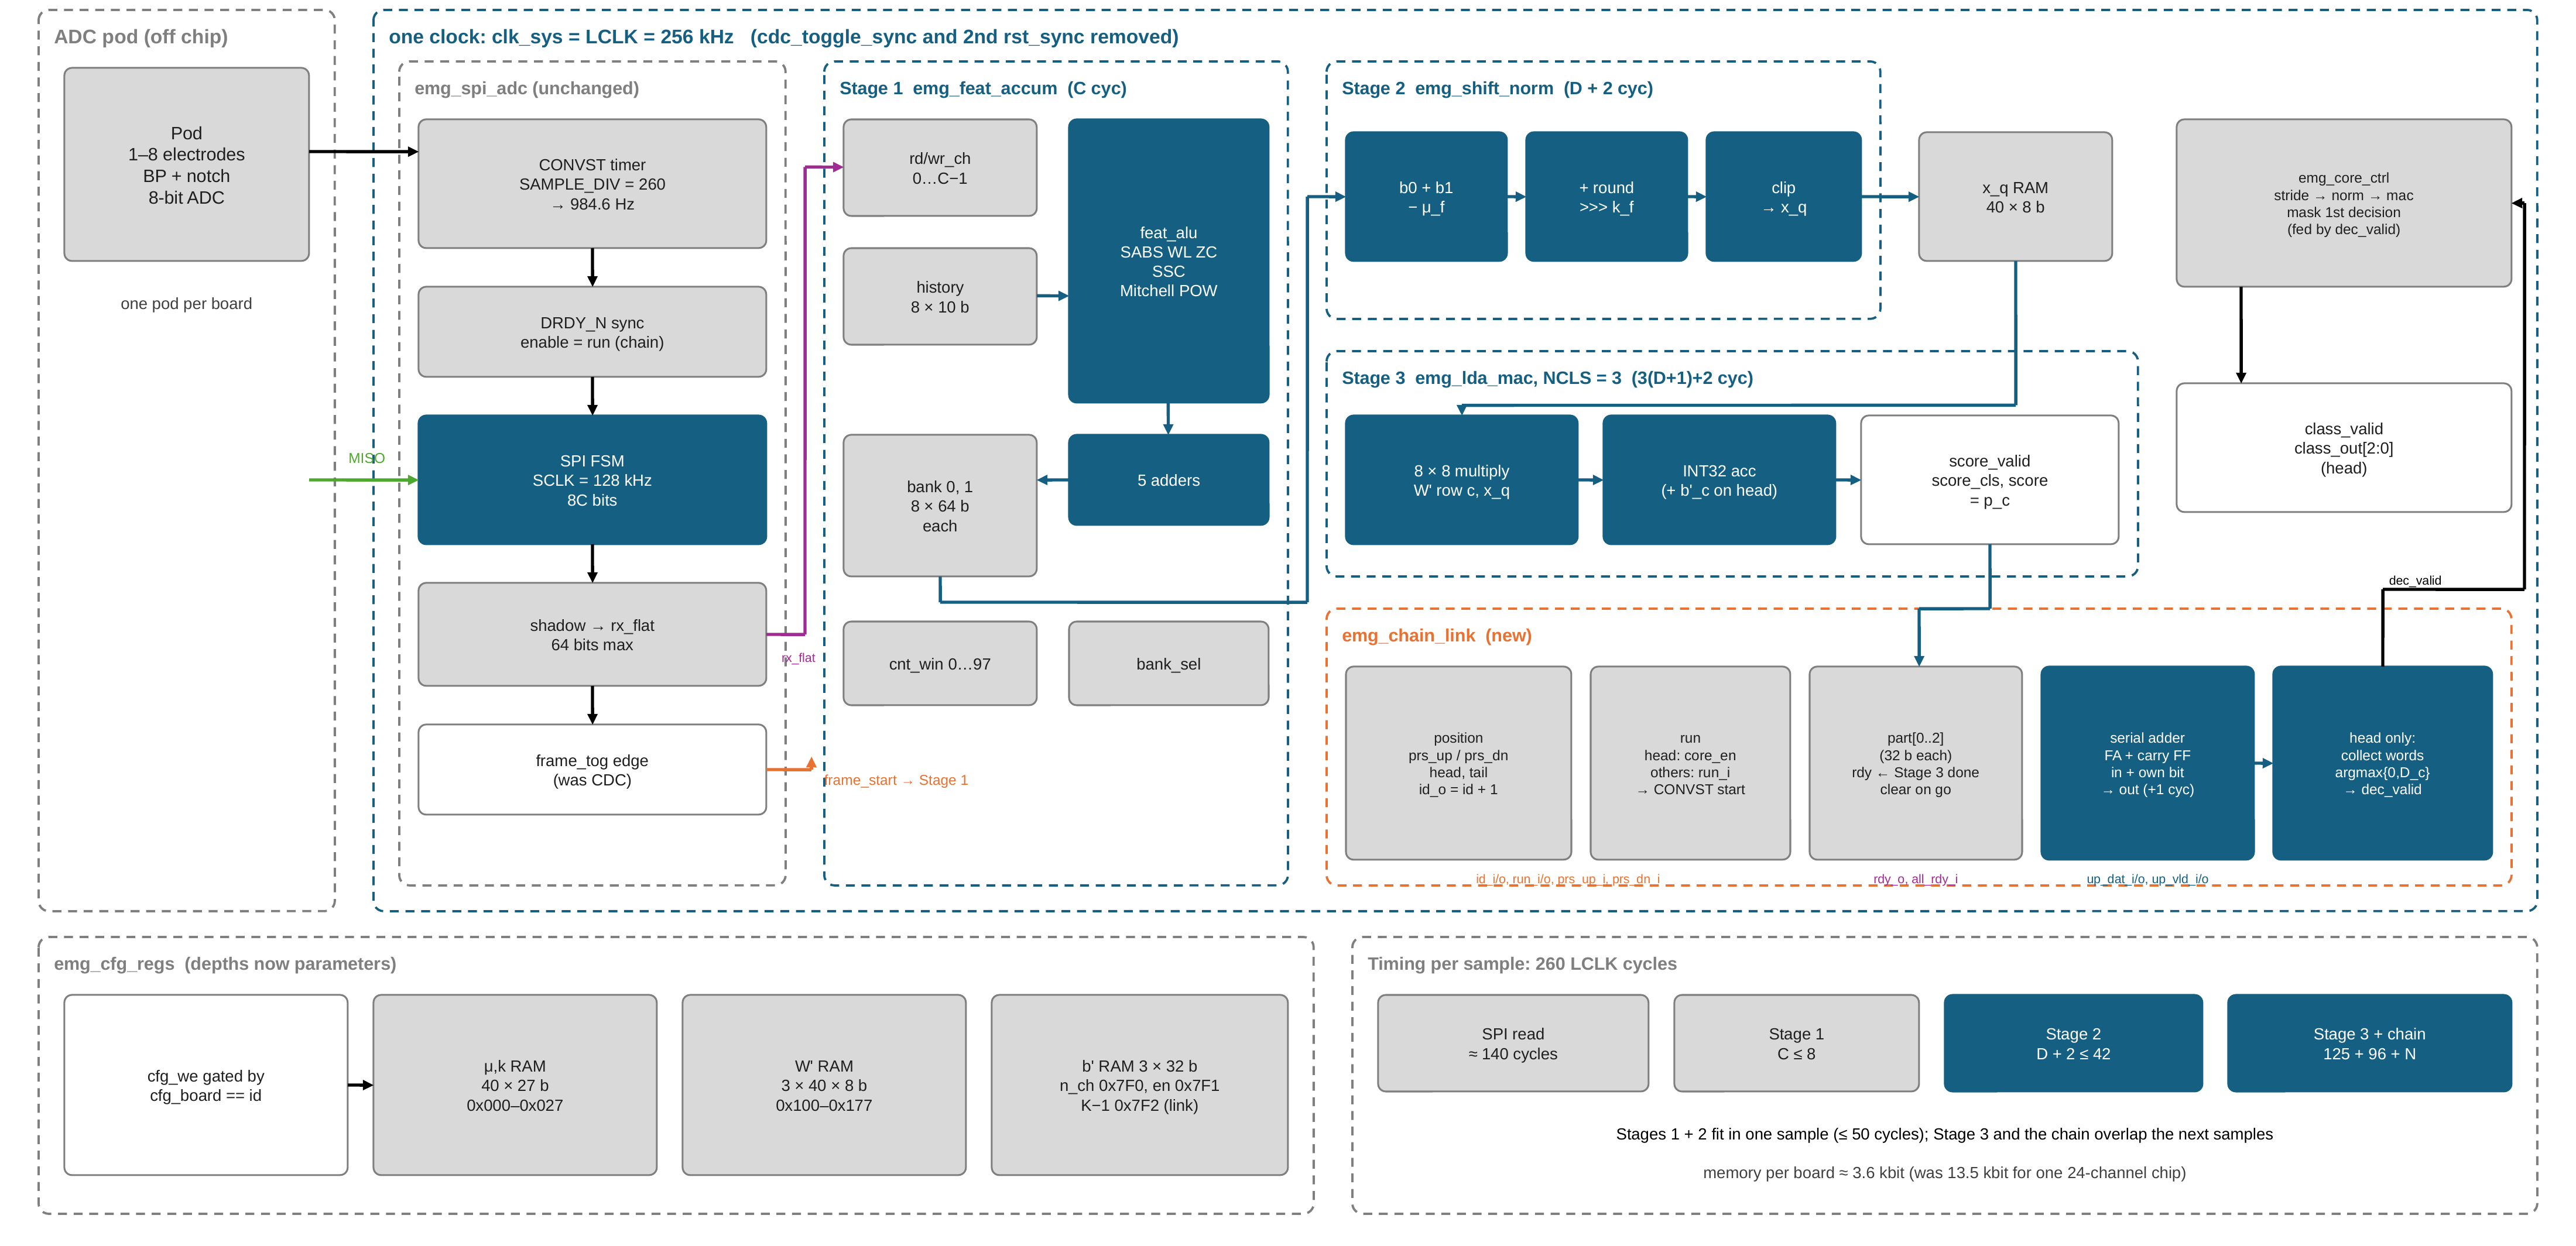
\includegraphics[width=\textwidth]{figures/board.png}
\caption{Datapath of one board with the RTL module names.}\label{fig:board}
\end{figure}

\begin{figure}[t]\centering
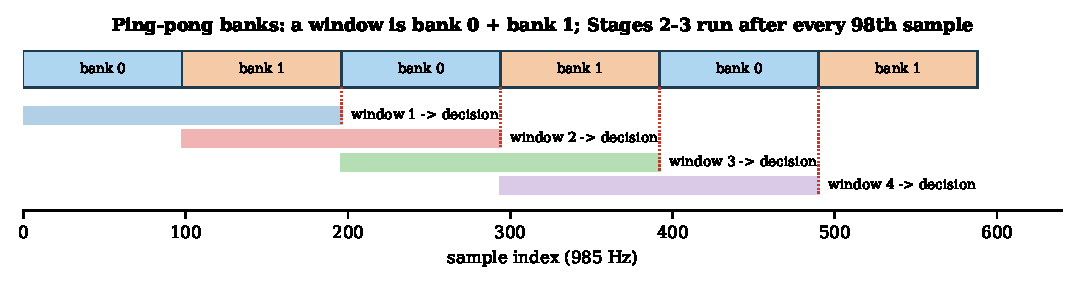
\includegraphics[width=\textwidth]{figures/banks.pdf}
\caption{Windowing with two banks. Each bank accumulates 98 samples; a window is the sum of the last two banks,
so each completed bank finishes a window and triggers one decision.}\label{fig:banks}
\end{figure}

\subsection{One clock: 256\,kHz}
The binding constraint is the ADC read. Eight channels of 8 bits at SCLK $=f_{\text{clk}}/2$ take 128 clock
cycles per sample, and the sample period is $1/985\,\text{Hz}\approx1.015$\,ms. At 128\,kHz the read alone would
fill the whole period, leaving no time for conversion and chip-select set-up. At 256\,kHz it takes about
0.5\,ms. The sample timer divides by 260, giving $256\,\text{kHz}/260=984.6$\,Hz, within 0.04\% of the
dataset's rate. Within one period, Stage 1 needs at most 8 cycles and, after the 98th sample, Stage 2 at most
42, so both finish long before the next frame (Figure~\ref{fig:timing}). Stage 3 and the chain transfer use only
the INT8 feature memory and the weights, so they overlap the next samples' reads. With eight channels per board
a decision is ready about 280 cycles ($\approx1.1$\,ms) after the last sample of a stride, out of 25{,}480 cycles
per stride: the datapath is idle about 99\% of the time, and one multiplier is enough.

One clock for every block and every board removes all clock-domain crossings, and boards cannot drift apart.
Against the single chip's 1\,MHz core and 8\,MHz interface, the dynamic power of the clock tree and the logic,
which scales with frequency, drops accordingly.

\begin{figure}[t]\centering
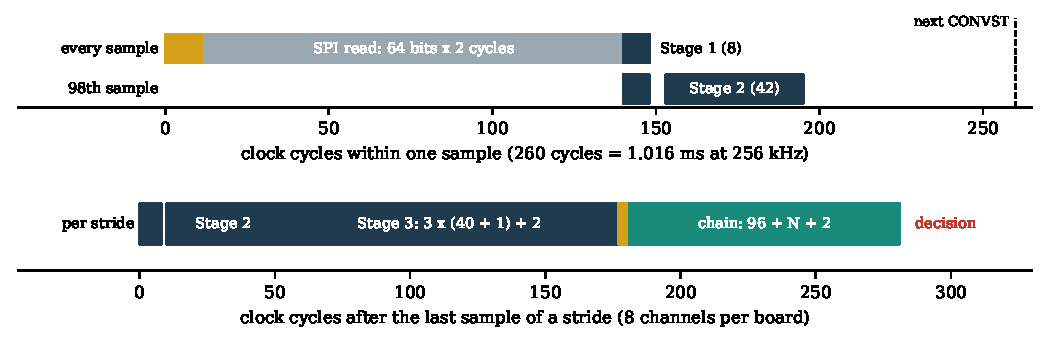
\includegraphics[width=\textwidth]{figures/timing.pdf}
\caption{Cycle budget at 256\,kHz. Top: one sample period. Bottom: the work after the last sample of a
stride.}\label{fig:timing}
\end{figure}

\subsection{Splitting the LDA across boards}\label{sec:split}
Let board $j$ own the feature set $F_j$, with $\bigcup_j F_j$ all $D$ features. The single-chip score of class
$c$ is a sum over features and therefore splits over boards:
\begin{equation}
s_c=\sum_{f}W_{cf}\,q_f+b_c=\sum_j\sum_{f\in F_j}W_{cf}\,q_f+b_c .
\end{equation}
Only the argmax is needed, and it is unchanged by subtracting the same number from every score:
\begin{equation}
\arg\max_c s_c=\arg\max\,\{0,\;s_1-s_0,\;s_2-s_0,\;s_3-s_0\}.
\end{equation}
So each board stores the $K-1$ difference rows $W'_c=W_c-W_0$ ($c=1,2,3$) for its own features and computes
\begin{gather}
p_c^{(j)}=\sum_{f\in F_j}W'_{cf}\,q_f\quad\big(+\,b'_c=b_c-b_0\ \text{on the head only}\big),\\
D_c=\sum_j p_c^{(j)},\qquad \hat c=\arg\max\,\{0,D_1,D_2,D_3\}.
\end{gather}
\begin{proposition}
If $D_c=s_c-s_0$ exactly for $c=1,\dots,K-1$, the chained decision equals the single-chip decision, including
ties, when both take the first maximum (strict $>$ in a running comparison).
\end{proposition}
\begin{proof}
The head starts the running comparison with best value $0$ and class $0$, which is the value $s_0-s_0$ of class
0, and then compares $D_1,\dots,D_{K-1}$ in order with strict $>$. This is the same sequence of comparisons as a
running argmax over $s_0,\dots,s_{K-1}$ shifted by the constant $-s_0$, so it selects the same index.
\end{proof}
In the hardware the difference rows are quantised directly to INT8 with one scale, rather than formed from the
INT8 single-chip rows, so the two quantised models are not bit-identical in general; on the real-data test stream
of Section~\ref{sec:verif} they agree on all 79 decisions. The scheme saves a quarter of the work: 120 instead of
160 MACs and weights for four classes, and 96 instead of 128 bits per decision on the chain. Whatever the channel
count of a board, it sends 96 bits per decision, compared with 320 bits for its INT8 features or 6{,}272 bits for
its raw samples.

\subsection{The chain protocol}\label{sec:chain}
The protocol needs no master and no per-board straps; every board runs the same logic.
\begin{enumerate}
\item \textbf{Position.} Two presence pins tell a board whether a neighbour exists upstream and downstream. A
board with nothing upstream is the head, one with nothing downstream the tail. The head has id 0; each board
passes $\text{id}+1$ downstream.
\item \textbf{Configuration.} A shared write bus carries address, data and a board number; a board accepts a
write only if the number equals its id. A four-plus-four split needs 171 writes (about 1.34\,ms).
\item \textbf{Start.} The last write sets the head's enable. It travels down the chain as a plain wire
(\texttt{run}), so every board's sample timer starts in the same clock cycle; with one shared clock the boards
then sample the same instant forever.
\item \textbf{Barrier.} Each board raises an open-drain ready line when its Stage 3 is done; the line is a
wired AND, high only when every board is ready. Its rising edge is \texttt{go} on every board in the same cycle,
and \texttt{ready} clears on \texttt{go}. Boards with fewer channels finish earlier and simply wait.
\item \textbf{Bit-serial sum.} The tail streams its three partial sums, 32 bits each, least significant bit
first. Every board adds its own bit with one full adder and a carry flip-flop and forwards the sum one cycle
later; the carry is cleared between words. The head shifts each completed total into a register and compares it
with the running best (strict $>$), so the decision is ready $96+N+2$ cycles after \texttt{go} for $N$ boards.
\end{enumerate}
Least-significant-bit-first order lets the carry ripple naturally, and two's-complement addition modulo $2^{32}$
is exact as long as every total stays within $\pm2^{31}$; measured scores are below $10^4$. Bit-serial transfer
needs two wires per link and a 1-bit adder per board, and takes 0.4\,ms of the 99.5\,ms stride.

\subsection{The design in operation}
Figures~\ref{fig:wave1}--\ref{fig:wave3} show the simulated waveforms of two boards (four channels each) on a
real FORS-EMG stream. At start-up (Figure~\ref{fig:wave1}) the reset is released at 20\,\textmu s, the boards
find their roles and ids from the presence pins, 171 configuration writes load both models, and the head's
enable starts both sample timers in the same cycle at 1.38\,ms. In steady state (Figure~\ref{fig:wave2}) the
boards only sample for 98 frames and then run one short burst per stride. Inside a stride
(Figure~\ref{fig:wave3}) Stage 2 takes 22 cycles, Stage 3 65 cycles, the barrier releases both boards together,
96 bits are added along the chain, and the head decides about 0.75\,ms after the last frame. In the stride shown,
the totals are $D=(742,-255,765)$, so the decision is class 3, as in the golden model.

\begin{figure}[p]\centering
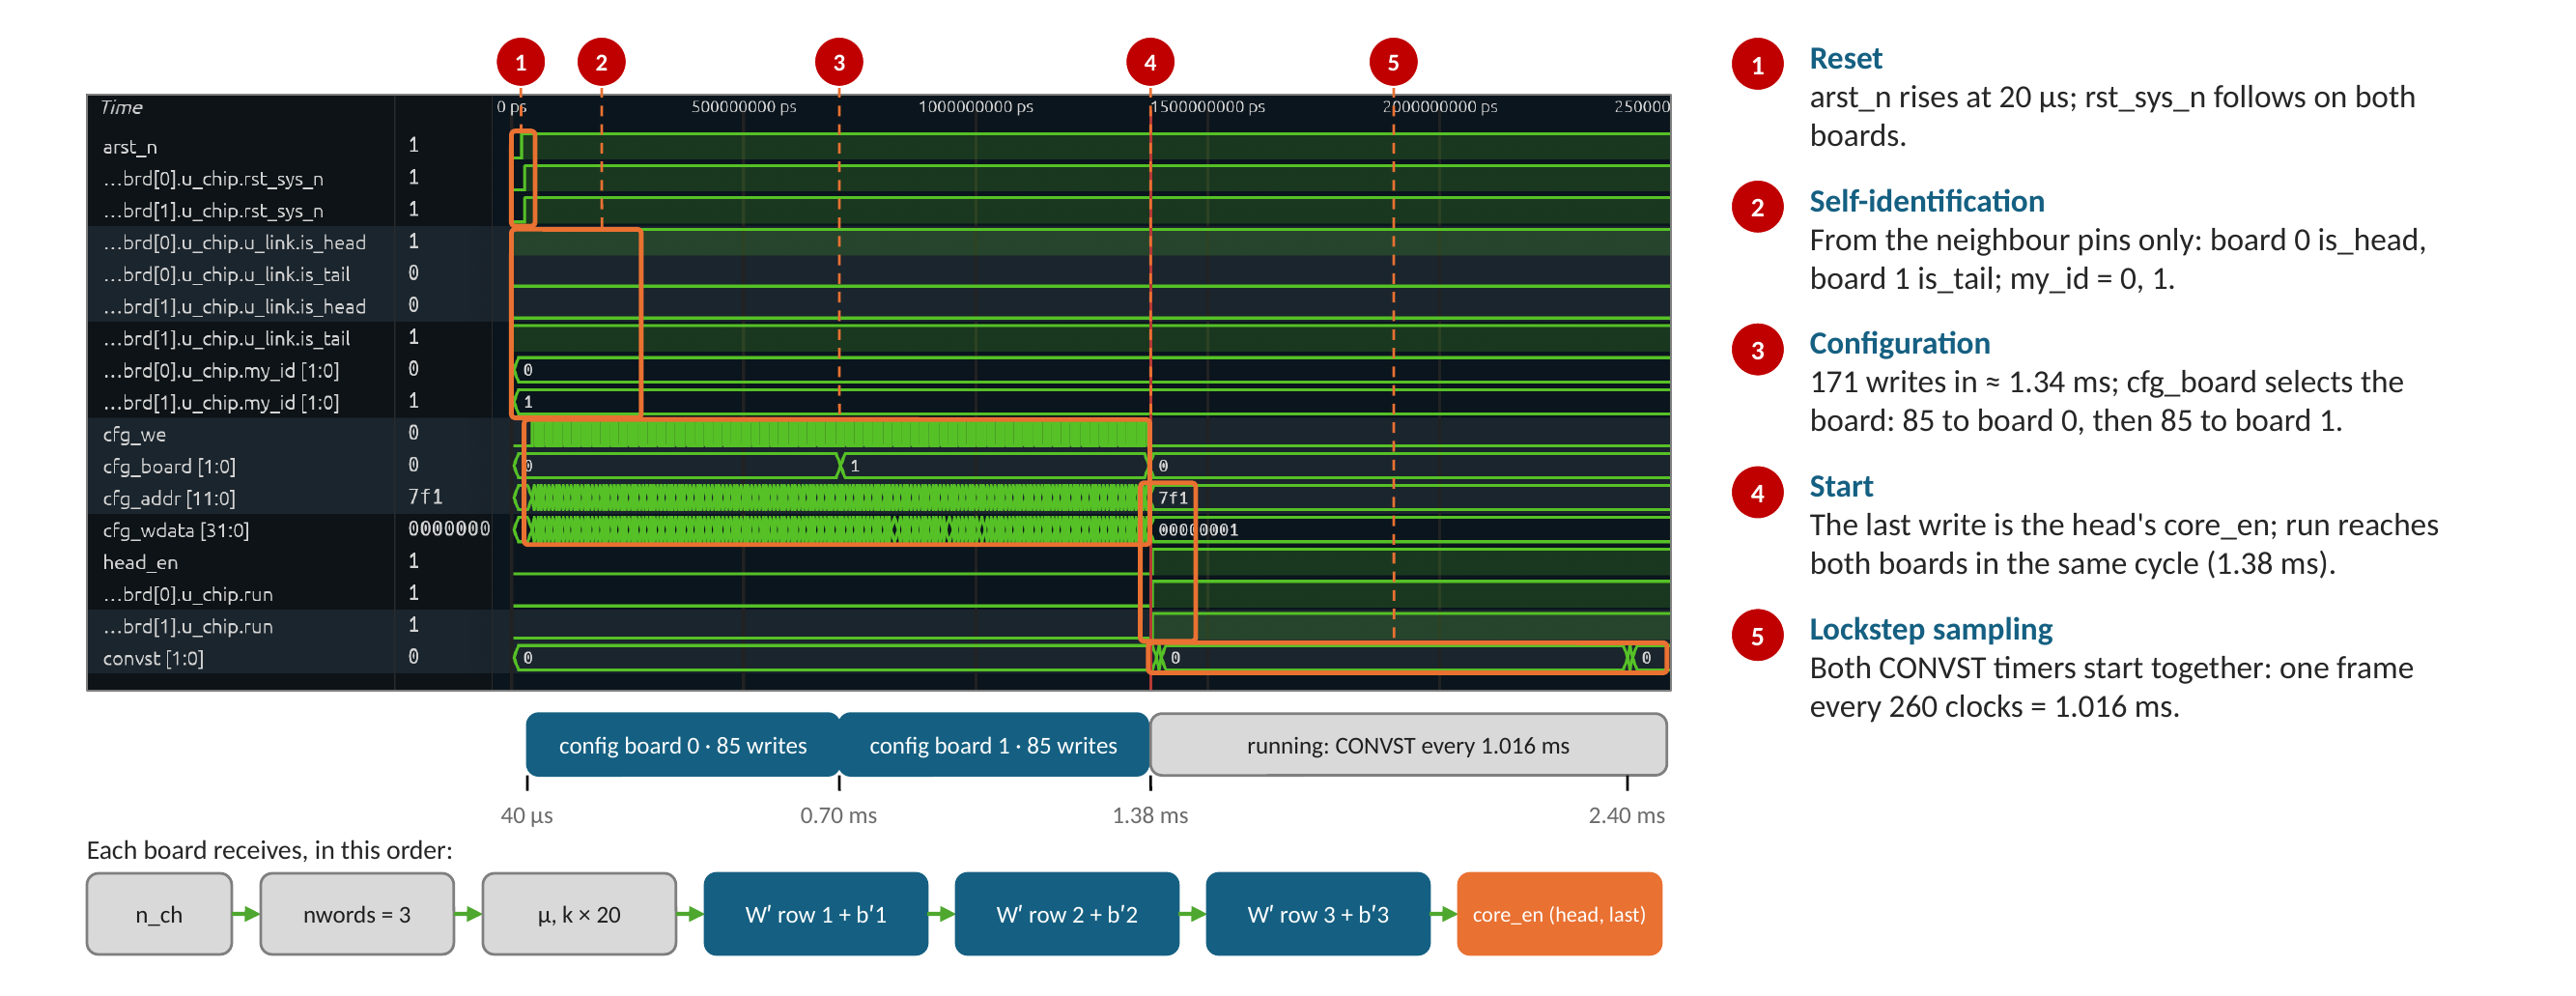
\includegraphics[width=\textwidth]{figures/wave_startup.png}
\caption{Start-up: reset, self-identification, configuration of board 0 then board 1, and the common start.}
\label{fig:wave1}
\vspace{6mm}
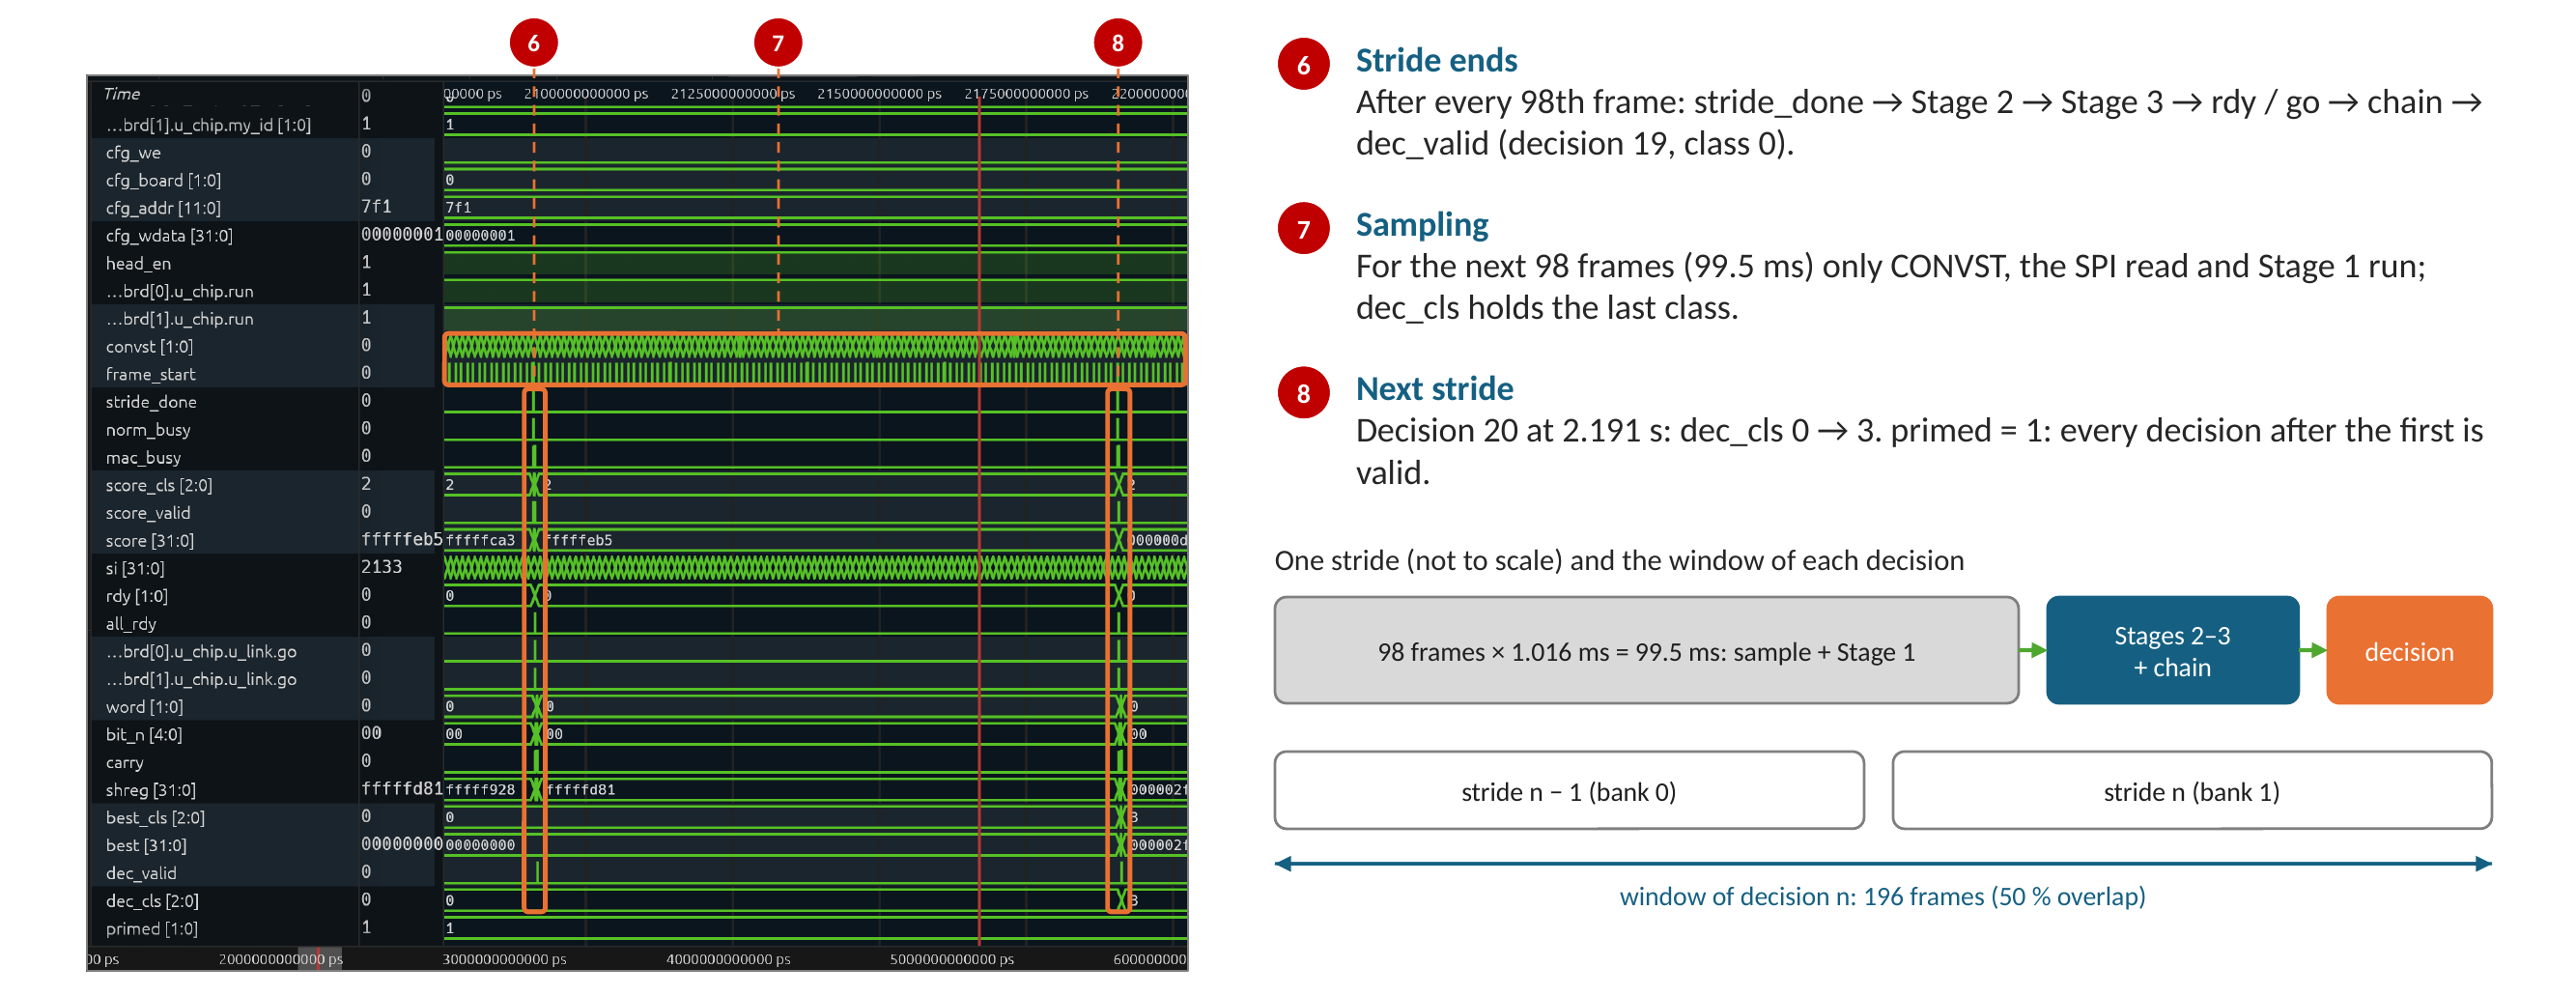
\includegraphics[width=\textwidth]{figures/wave_strides.png}
\caption{Steady state: continuous sampling and one burst of work per stride (two strides shown).}\label{fig:wave2}
\end{figure}

\begin{figure}[t]\centering
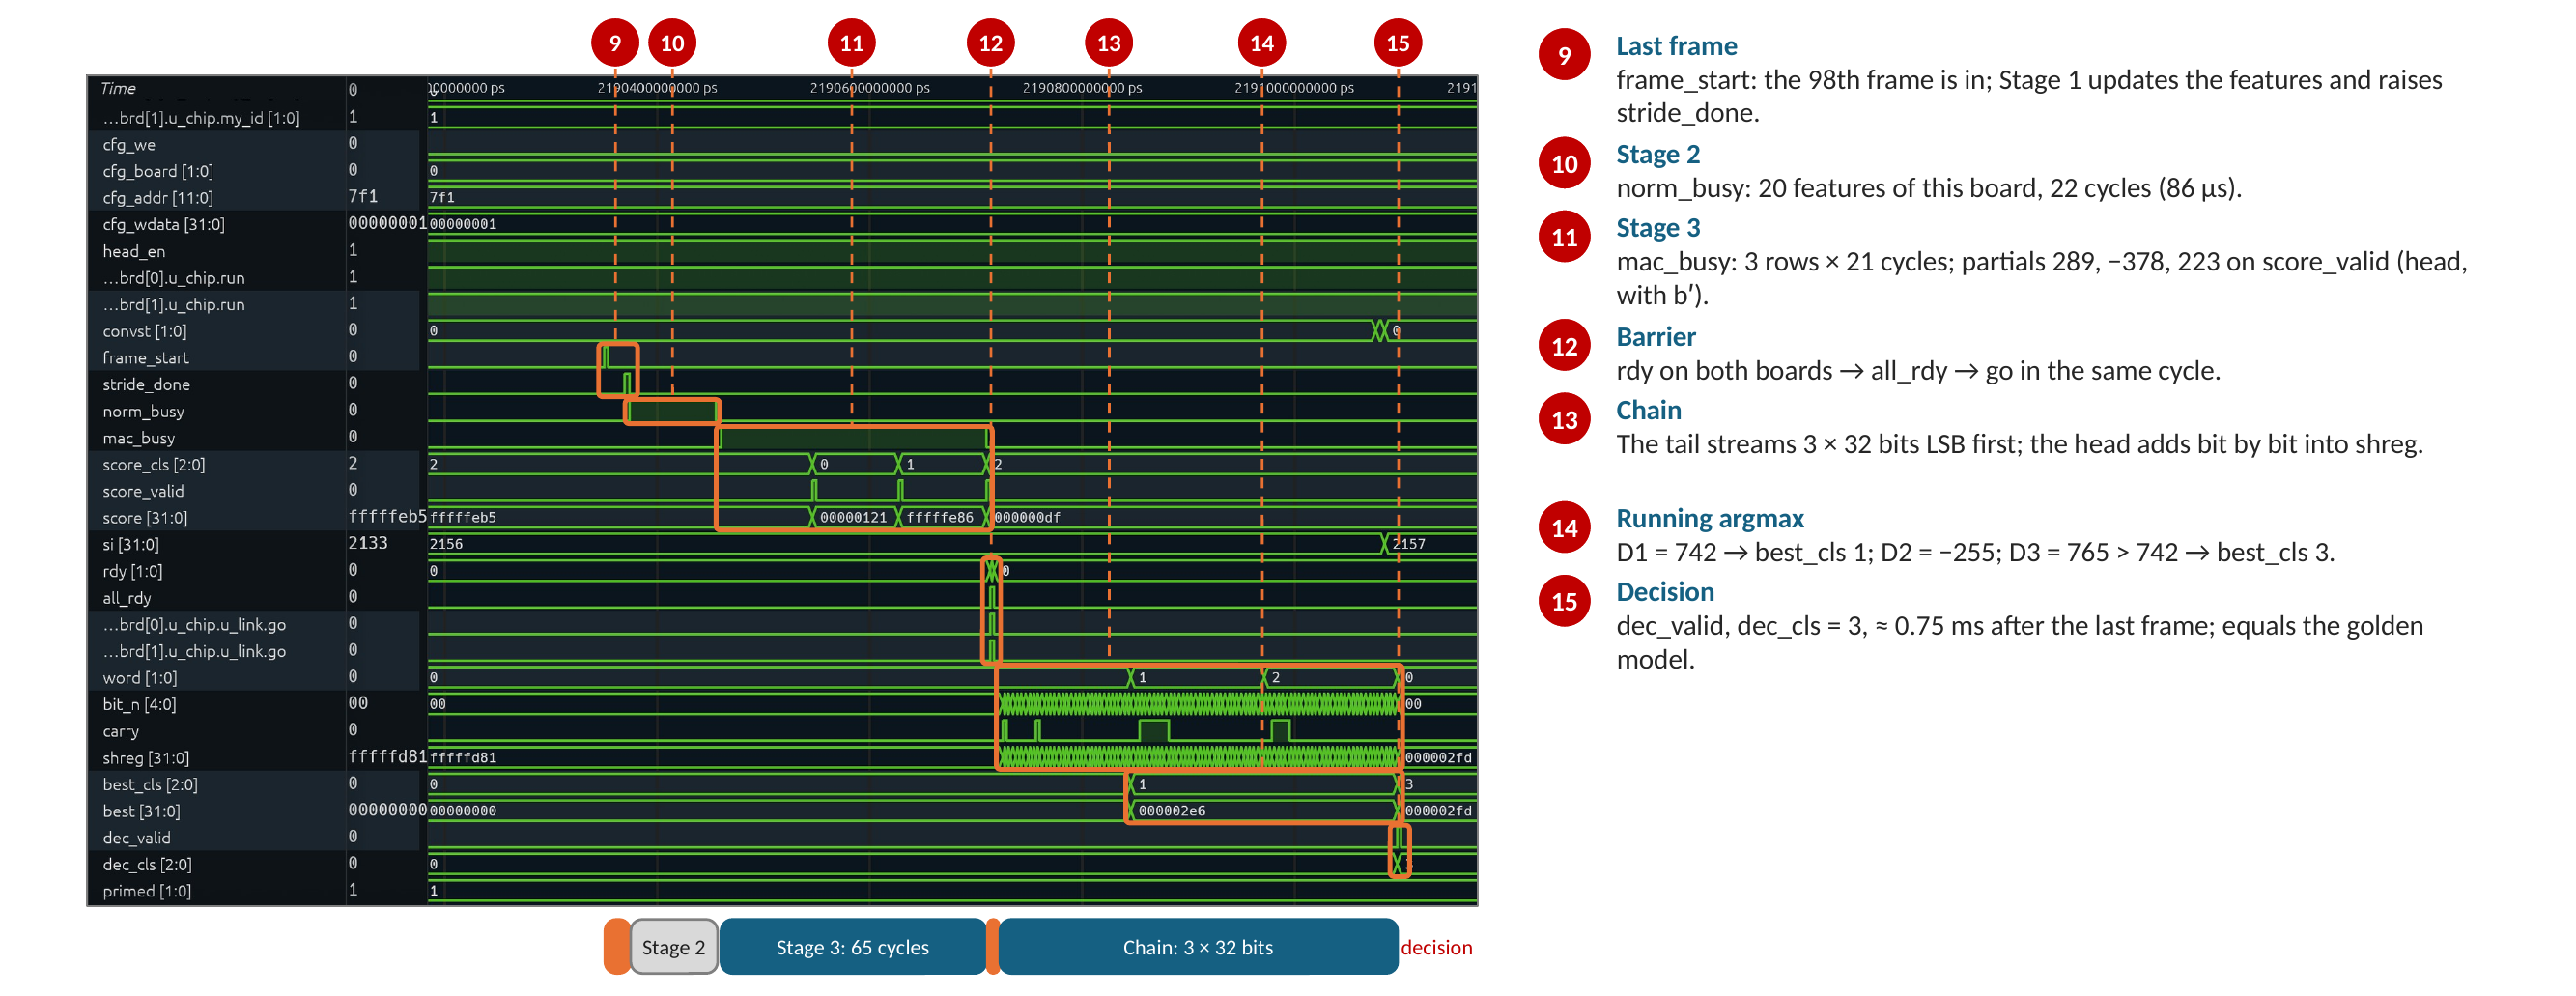
\includegraphics[width=\textwidth]{figures/wave_stride.png}
\caption{Inside one stride, from the last frame to the decision.}\label{fig:wave3}
\end{figure}

%==========================================================================================
\section{Verification}\label{sec:verif}
\paragraph{Golden model.} A Python model reproduces every integer of Stages 1--3 in two forms, a
sample-by-sample model that mirrors the RTL's counters and a vectorised model used for training; the two are
cross-checked on every run. Training uses the model's own bit-exact features, so training and hardware see
identical numbers.

\paragraph{Chain link alone.} A self-checking testbench drives one to four chain links with random partial sums
(large, small, strictly negative and forced ties) for 3000 strides each, with $K-1=3$, 2 and 1 rows, and with a
random finishing time per board. It computes the expected totals and argmax itself, independently of the Python
model, and checks that exactly one decision appears at the head, with the right class, and none elsewhere.

\paragraph{Mutation test.} A testbench is trustworthy only if it fails on wrong hardware. Eight bugs were planted
one at a time: carry not cleared between words, adder ignoring the carry, ties going to the higher class, last
word dropped, decision using a stale best class, class-0 baseline not reset, ready never cleared, ids not
incremented. The unit test fails on every one.

\paragraph{Whole chip on real data.} One to three boards, each with a behavioural ADC pod, are fed subject 6,
trial 1 of FORS-EMG (the most active 1960 samples of each of the four gestures, 7840 samples), with a model
trained on the other subjects. For the splits 8, 4+4, 2+6, 6+2, 5+3 and 3+3+2 channels, all 79 decisions equal
the golden model bit for bit, and the golden multi-board decisions equal the single-chip LDA on all 79.
On windows that contain a single gesture, 72 of 76 decisions are correct; the four errors are the model's own.
All 18 checks pass (4 unit, 8 mutants, 6 splits). The single-chip predecessor was verified bit-exactly at 8, 12,
16, 20 and 24 channels with a chip-level cocotb test, and its feature ALU exhaustively on all 196{,}608 input
combinations.

\paragraph{Bugs found.} The whole-chip test found one real bug: clearing \texttt{ready} on a board's own end of
Stage 3 let a fast board raise it again while a slow board's old \texttt{ready} was still high, so uneven splits
produced two decisions per stride. Clearing on \texttt{go} fixed it. A testbench bug (counting the reset
transition as a sample) was also found and fixed.

%==========================================================================================
\section{Limitations}\label{sec:limits}
\begin{itemize}
\item \textbf{Closed vocabulary.} The classifier always answers one of four gestures and has no rest or reject
class; a movement outside the set is forced into one of them. FORS-EMG has no rest recordings.
\item \textbf{Selection on test folds.} The ranking of gesture subsets used confusion matrices that include the
test subjects (Section~\ref{sec:merge}), which is mildly optimistic for set D; the merge comparison is free of
this.
\item \textbf{One session per subject.} Day-to-day changes, electrode shift, fatigue and force variation are not
measured. Arm-position robustness was measured only in the CNN study.
\item \textbf{Different settings.} The LDA calibration of Section~\ref{sec:calib} (four gestures, 18 subjects,
fixed $\lambda=0.5$) and the CNN checkpoint (six groups, held windows, blend chosen on validation, 19
subjects) use different settings; each comparison is paired within its own setting, but their absolute numbers
should not be compared with each other.
\item \textbf{Multiple comparisons.} Paired tests are reported per question without correction for the number of
comparisons; every decision rests on intervals well away from zero or on non-inferiority.
\item \textbf{Simulation only.} The design is verified in RTL simulation with behavioural ADC pods. Area and power
in a target process, and tests with real pods and electrodes, remain to be done.
\end{itemize}

%==========================================================================================
\section{Conclusion}
For subject-independent sEMG gesture recognition with eight surface electrodes, the vocabulary decides more than
the model: choosing gestures driven by distinct, superficial muscles gains 14\pp, and keeping every gesture by
merging loses 17\pp. Model capacity adds little: linear models tie with an MLP, and a raw-signal CNN gains at most
2.7\pp\ before and 2.4\pp\ after calibration, at three orders of magnitude more arithmetic. An integer-only front
end and INT8 weights cost nothing, and one calibration recording per gesture is worth more than any model change.
These findings allow a very small machine: identical boards with eight channels, one 256\,kHz clock, one
multiplier and 3.7\,kbit of memory each, exchanging 96 bits per decision, verified bit-exactly on real data. Next
steps are on-chip calibration of the class means, robustness to forearm rotation, a rest class, and synthesis.

%==========================================================================================
\appendix
\section{Reproducing the results}
All scripts are in the project repository and print their results; they write no files.
\begin{center}\small
\begin{adjustbox}{max width=\textwidth}
\begin{tabular}{p{4.6cm}p{8.6cm}l}\toprule
Result & Script & Subjects\\\midrule
Gesture sets, classifiers, INT8 loss & \texttt{analysis/classifier\_classification.py},\newline \texttt{K\_4\_model\_MLP.py}, \texttt{K\_6\_model\_LR\_comparison.py} & 19\\
Merging versus dropping & \texttt{analysis/K\_4\_LDA\_Merge\_vs\_Drop.py} & 19\\
Feature-type selection & \texttt{analysis/fors\_emg\_feature\_selection\_lda.py} & 18\\
Integer features H1--H6 & \texttt{analysis/K\_4\_LDA\_HW\_Experiments.py} & 18\\
Chip model vs software LDA & \texttt{golden\_model/K\_4\_LDA\_Golden\_LOSO.py} & 18\\
CNNs vs LDA & \texttt{analysis/K\_4\_CNN\_LOSO.py} & 19\\
LDA and CNN calibration & \texttt{analysis/K\_4\_LDA\_Calib.py}, \texttt{K\_4\_CNN\_Calib.py} & 18\\
Multi-board RTL verification & \texttt{RTL/tb/verify\_all.py} & real data, subject 6\\\bottomrule
\end{tabular}
\end{adjustbox}
\end{center}

\begin{thebibliography}{10}\small
\bibitem{forsemg} \emph{FORS-EMG: A Novel sEMG Dataset for Hand Gesture Recognition Across Multiple Forearm
Orientations}, arXiv:2409.07484, 2024.
\bibitem{hudgins1993} B.~Hudgins, P.~Parker, R.~N.~Scott, ``A new strategy for multifunction myoelectric
control,'' \emph{IEEE Trans.\ Biomed.\ Eng.}, vol.~40, no.~1, pp.~82--94, 1993.
\bibitem{englehart2003} K.~Englehart, B.~Hudgins, ``A robust, real-time control scheme for multifunction
myoelectric control,'' \emph{IEEE Trans.\ Biomed.\ Eng.}, vol.~50, no.~7, pp.~848--854, 2003.
\bibitem{scheme2011} E.~Scheme, K.~Englehart, ``Electromyogram pattern recognition for control of powered
upper-limb prostheses: state of the art and challenges for clinical use,'' \emph{J.\ Rehabil.\ Res.\ Dev.},
vol.~48, no.~6, pp.~643--659, 2011.
\bibitem{phinyomark2012} A.~Phinyomark, P.~Phukpattaranont, C.~Limsakul, ``Feature reduction and selection for
EMG signal classification,'' \emph{Expert Syst.\ Appl.}, vol.~39, no.~8, pp.~7420--7431, 2012.
\bibitem{fougner2011} A.~Fougner, E.~Scheme, A.~D.~C.~Chan, K.~Englehart, \O.~Stavdahl, ``Resolving the limb
position effect in myoelectric pattern recognition,'' \emph{IEEE Trans.\ Neural Syst.\ Rehabil.\ Eng.}, vol.~19,
no.~6, pp.~644--651, 2011.
\bibitem{farrell2007} T.~R.~Farrell, R.~F.~Weir, ``The optimal controller delay for myoelectric prostheses,''
\emph{IEEE Trans.\ Neural Syst.\ Rehabil.\ Eng.}, vol.~15, no.~1, pp.~111--118, 2007.
\bibitem{jacob2018} B.~Jacob \emph{et al.}, ``Quantization and training of neural networks for efficient
integer-arithmetic-only inference,'' in \emph{Proc.\ IEEE CVPR}, 2018, pp.~2704--2713.
\bibitem{mitchell1962} J.~N.~Mitchell, ``Computer multiplication and division using binary logarithms,''
\emph{IRE Trans.\ Electron.\ Comput.}, vol.~EC-11, no.~4, pp.~512--517, 1962.
\bibitem{ledoit2004} O.~Ledoit, M.~Wolf, ``A well-conditioned estimator for large-dimensional covariance
matrices,'' \emph{J.\ Multivariate Anal.}, vol.~88, no.~2, pp.~365--411, 2004.
\end{thebibliography}
\end{document}
